\documentclass[12pt,a4paper]{article}

\usepackage[T1]{fontenc}
\usepackage[utf8]{inputenc}
\usepackage{lmodern}
\usepackage{geometry}
\usepackage{setspace}
\usepackage{amsmath,amssymb}
\usepackage{booktabs}
\usepackage{array}
\usepackage{tabularx}
\usepackage{graphicx}
\usepackage{caption}
\usepackage{subcaption}
\usepackage{enumitem}
\usepackage{xcolor}
\usepackage{listings}
\usepackage{indentfirst}
\usepackage{placeins}
\usepackage[numbers,sort&compress]{natbib}
\usepackage{hyperref}

\geometry{left=2.6cm,right=2.4cm,top=2.5cm,bottom=2.5cm}
\onehalfspacing
\setlength{\parindent}{1.1cm}
\setlength{\parskip}{0pt}
\setlength{\emergencystretch}{2em}
\setlist[itemize]{leftmargin=1.2cm,itemsep=0.1\baselineskip,topsep=0.2\baselineskip}
\setlist[enumerate]{leftmargin=1.2cm,itemsep=0.1\baselineskip,topsep=0.2\baselineskip}
\setcounter{topnumber}{3}
\setcounter{bottomnumber}{2}
\setcounter{totalnumber}{5}
\setcounter{tocdepth}{2}
\renewcommand{\topfraction}{0.92}
\renewcommand{\bottomfraction}{0.82}
\renewcommand{\textfraction}{0.08}
\renewcommand{\floatpagefraction}{0.82}

\hypersetup{
  colorlinks=true,
  linkcolor=blue,
  citecolor=blue,
  urlcolor=blue
}
\captionsetup{font=small,labelfont=bf}
\lstdefinestyle{rcode}{
  basicstyle=\ttfamily\footnotesize,
  breaklines=true,
  frame=single,
  columns=fullflexible,
  keepspaces=true,
  showstringspaces=false,
  backgroundcolor=\color{black!3},
  rulecolor=\color{black!25},
  xleftmargin=0.4cm,
  xrightmargin=0.4cm
}

\newcolumntype{L}[1]{>{\raggedright\arraybackslash}p{#1}}
\newcolumntype{C}[1]{>{\centering\arraybackslash}p{#1}}
\newcommand{\bp}{\mathrm{bp}}
\newcommand{\OFI}{\mathrm{OFI}}
\newcommand{\Prob}{\mathbb{P}}
\newcommand{\E}{\mathbb{E}}
\newcommand{\doi}[1]{\href{https://doi.org/#1}{doi:#1}}
\newcommand{\tabref}[1]{\hyperref[#1]{Table~\ref*{#1}}}
\newcommand{\apptabref}[1]{\hyperref[#1]{Appendix Table~\ref*{#1}}}
\newcommand{\figref}[1]{\hyperref[#1]{Figure~\ref*{#1}}}
\newcommand{\appfigref}[1]{\hyperref[#1]{Appendix Figure~\ref*{#1}}}
\newcommand{\secref}[1]{\hyperref[#1]{Section~\ref*{#1}}}

\title{Regime-Dependent Price Impact in the MOEX Limit Order Book}
\author{Nikolay Tagin}
\date{May 2026}

\begin{document}

\maketitle

\begin{abstract}
\hspace*{\parindent}This paper studies whether short-horizon price impact in the Moscow Exchange limit order book depends on the liquidity state of the market. This question matters because average intraday regressions can hide short periods when the book becomes expensive and fragile. I reconstruct top-of-book quotes and order-flow imbalance (OFI) from MOEX Full Orders Log data for 15 blue-chip equities from April to June 2025, then estimate a three-state hidden Markov model on 30-second stock-day sequences. The emissions equation combines de-seasonalized relative spreads and winsorized midprice returns, with a state-specific slope on depth-scaled OFI. The model identifies Calm, Normal  and Stressed liquidity-cost regimes. The Stressed regime has the widest spread and thinnest displayed book, but it is not the highest-volatility state. It is more naturally read as liquidity withdrawal than active panic. The price-impact point estimates differ by almost two orders of magnitude between Calm and Stressed. A covariate-transition version of the model shows that lower depth predicts entry into the Stressed state, while higher depth predicts recovery.
\end{abstract}

\begin{center}
\small
\textbf{Replication repository:}\\
\resizebox{0.95\textwidth}{!}{\href{https://github.com/nikolajtagin/regime-dependent-price-impact-in-the-moex-limit-order-book}
{\texttt{github.com/nikolajtagin/regime-dependent-price-impact-in-the-moex-limit-order-book}}}\\
The public repository contains the numbered R scripts and generated results used for the tables and figures.
\end{center}

\clearpage
\tableofcontents
\clearpage

\section{Introduction}\label{sec:introduction}

The main result is that intraday price impact varies strongly across liquidity states. In the MOEX limit order book, the point estimates imply that a one-standard-deviation shock to depth-scaled order-flow imbalance moves prices far more in the Calm state than in the Stressed state. A single average price-impact coefficient would miss this difference.

This is why a regime model is useful here. Liquidity changes minute by minute as quoted spreads, visible depth  and order flow move together. A non-homogeneous HMM lets the model learn hidden states from spreads and returns and then links state transitions to current order-book conditions. In practical terms, it asks what liquidity state the book is in now and which observed conditions make the next state more likely.

I bring these ideas to an intraday equity setting. The empirical sample covers 15 MOEX Blue Chip stocks from April 1 to June 30, 2025. I estimate a non-homogeneous hidden Markov model (NHMM) on 955,110 observations, organized as 930 stock-day sequences on a 30-second grid. ``Non-homogeneous'' means that transition probabilities are allowed to change with market conditions instead of being fixed for the whole sample. The emissions are bivariate: de-seasonalized relative spread and winsorized midprice return are modeled jointly, with a state-specific return slope on depth-scaled OFI. Transition probabilities depend on de-seasonalized depth, realized volatility (RV), absolute OFI pressure  and open/close indicators.

The paper makes three empirical points. The OFI-return slope is strongly state-dependent: the point estimates are 43.5 basis points in Calm, 5.8 in Normal  and close to zero in Stressed for a one-standard-deviation OFI shock. Stressed is not the high-volatility regime: quotes widen and depth thins, but realized volatility is closer to Calm and the OFI-return slope is near zero. Depth has the largest and most precisely estimated marginal effect in the transition model: low depth predicts entry into Stressed, while higher depth predicts recovery.

I use the HMM for economic description rather than forecast benchmarking. States are not labelled before estimation. I estimate them and then assign labels by ranking the estimated spread intercepts. The transition covariates are also interpreted carefully. Depth, realized volatility  and order-flow pressure are market outcomes as well as predictors, so the coefficients are predictive associations rather than causal effects.

The remainder of the paper covers the literature, data and variables, the HMM specification, diagnostics, results, robustness  and conclusion.

\section{Literature and Economic Mechanism}\label{sec:literature}

\subsection{Liquidity, order flow  and price impact}\label{sec:literature_liquidity}

Market liquidity has several dimensions. The spread measures tightness, depth measures visible quantity  and price impact measures resiliency. Classic adverse-selection models explain why spreads widen when liquidity providers fear informed trading \citep{GlostenMilgrom1985,EasleyOHara1992}. \citet{Kyle1985} gives the standard price-impact interpretation: a higher \(\lambda\) means that a given signed order-flow shock moves prices more strongly. Empirically, \citet{Hasbrouck1991} shows that trades contain information about later price movements  and \citet{LeeReady1991} provides a widely used approach for inferring trade direction in intraday data.

The order-book reference most directly used in this paper is \citet{ContKukanovStoikov2014}. They show that short-horizon price changes are mainly driven by order-flow imbalance at the best bid and ask  and that the slope is approximately inversely proportional to market depth. This is why the emission equation uses depth-scaled OFI rather than signed trade volume alone. The estimated \(\lambda_i\) should therefore be read as a local price-sensitivity measure inside a 30-second bucket. It is not a full theory of large institutional execution.

\subsection{Dynamic liquidity and fragility}\label{sec:literature_fragility}

Liquidity is persistent and state-dependent. \citet{AndersenBollerslev1997} document strong intraday periodicity in volatility. \citet{ChordiaRollSubrahmanyam2000} show commonality in liquidity, which supports looking for market-wide liquidity states rather than only isolated stock-level episodes. \citet{NguyenEngleFlemingGhysels2020} model intraday liquidity, volume  and volatility jointly in the U.S. Treasury market. Their paper is a useful benchmark because it treats liquidity and volatility as connected intraday objects rather than separate daily summaries.

The closest motivation is liquidity fragility. \citet{MeldrumSokolinskiy2025} study Treasury markets and show that lower market depth increases the fragility of liquidity. The intuition is direct: when few resting orders are visible, the market depends more on quick replenishment. If that replenishment slows down, liquidity can deteriorate even before a large price move is observed. I apply a related hidden-state idea to intraday equity order books and add a regime-specific OFI-return slope, so the model links quoted costs, displayed depth  and short-horizon price sensitivity in the same framework.

The liquidity-withdrawal interpretation also connects to theory and evidence on adverse selection and liquidity provision. \citet{FoucaultKadanKandel2005} model the limit order book as a market where patient traders provide liquidity and impatient traders demand it. \citet{BrunnermeierPedersen2009} show how market liquidity and funding liquidity can reinforce each other, generating liquidity spirals. \citet{CespaFoucault2014} show how illiquidity can propagate through cross-asset learning. \citet{RamanRobeYadav2020} document that algorithmic liquidity providers can reduce liquidity supply in stressful periods.

\subsection{Latent regimes}\label{sec:literature_regimes}

Hidden Markov models are useful when observed variables are driven by a small number of unobserved states. \citet{Hamilton1989} is the canonical reference for Markov-switching methods in economics. In liquidity applications, \citet{FloodLiechtyPiontek2016} use hidden Markov chains to identify common liquidity regimes across markets.

I use a custom HMM implementation because the emission equation combines a bivariate state-dependent distribution with a state-specific price-impact slope. I then use an NHMM because a constant-transition HMM can say that regimes exist, but it cannot say which current market conditions make entry into or exit from Stressed more likely. The goal is a compact economic description of intraday liquidity-cost regimes and the conditions associated with transitions between them.

\section{Data and Variable Construction}\label{sec:data}

\subsection{Sample}\label{sec:sample}

The empirical sample is the MOEX Blue Chip equity universe over April 1--June 30, 2025. MOEX describes the Blue Chip Index as a price-return index composed of 15 liquid Russian equity-market stocks, with constituents revised quarterly \citep{MOEXBlueChip}. The sample contains the following securities:
\begin{center}
\small\setlength{\tabcolsep}{12pt}
\begin{tabular}{lllll}
\texttt{CHMF} & \texttt{GAZP} & \texttt{GMKN} & \texttt{HEAD} & \texttt{LKOH} \\
\texttt{MOEX} & \texttt{NLMK} & \texttt{NVTK} & \texttt{PLZL} & \texttt{ROSN} \\
\texttt{SBER} & \texttt{SNGS} & \texttt{T} & \texttt{TATN} & \texttt{YDEX}
\end{tabular}
\end{center}
The main continuous session is 10:00:00--18:39:59 Moscow time. Weekends are excluded. The primary HMM sample contains 62 calendar trading days, 15 stocks, 930 stock-day sequences  and 955,110 final 30-second observations.

MOEX has a brief intraday clearing session at 14:00--14:05 Moscow time. The resulting spread spike and dip in trade activity are removed from the modeled spread and depth levels by within-stock five-minute time-of-day demeaning, but the pattern remains visible in the raw intraday profiles reported in the appendix.

\begin{table}[!htbp]
\centering
\caption{Sample construction}
\small
\begin{tabular}{L{0.45\textwidth}r}
\toprule
\textbf{Object} & \textbf{Value} \\
\midrule
Stocks & 15 \\
Calendar trading days & 62 \\
Stock-day sequences & 930 \\
Primary frequency & 30 seconds \\
Final HMM observations & 955,110 \\
Observations per stock & 63,674 \\
Main session & 10:00--18:39:59 \\
Raw reconstruction grid & 5 seconds \\
Response variable & Winsorized midprice return \\
Flow variable & Depth-scaled OFI \\
\bottomrule
\end{tabular}
\caption*{\footnotesize\emph{Notes:} The table is based on the model-ready 30-second panel generated by the data-construction scripts. Each stock-day is treated as a separate HMM sequence, so overnight gaps and cross-stock boundaries are not modeled as ordinary 30-second transitions.}
\label{tab:sample}
\end{table}

The empirical pipeline is fully reproducible from the numbered R scripts in the \href{https://github.com/nikolajtagin/regime-dependent-price-impact-in-the-moex-limit-order-book}{public replication repository}. Script 01 stores shared settings and functions. Script 02 reconstructs the top of the book from event-level MOEX order logs. Script 03 combines stock-day files into the primary 30-second panel and robustness samples. Script 04 produces diagnostics on seasonality, stationarity, normality, regressors  and price impact. Script 05 estimates the one-state benchmark, the constant-transition HMM, the NHMM, compact posterior diagnostics  and bootstrap average marginal effects. Script 06 estimates the robustness models.

\subsection{Order-book reconstruction}\label{sec:reconstruction}

The raw data are MOEX Full Orders Log files. The file layout includes order number, side, event action, price, volume, trade number  and trade price fields \citep{MOEXFullOrdersLog}. The reconstruction code streams the order log security by security and keeps an active visible book indexed by order number. A placement adds visible limit order volume to the book. A cancellation removes the remaining visible volume. A trade reduces the volume of the resting order that was executed. After each event, the best bid and ask are read from the active price-level maps.

Let \(b_t\) and \(a_t\) denote the best bid and ask at the end of bucket \(t\). Let \(D^{bid}_t\) and \(D^{ask}_t\) be the displayed quantities available at those two best quotes. The midprice, spread  and total top-of-book depth are
\[
m_t=\frac{a_t+b_t}{2}, \qquad
s_t=a_t-b_t, \qquad
D_t=D^{bid}_t+D^{ask}_t .
\]
Thus \(D_t\) is not total market depth at all price levels. It is only the volume visible at the best bid plus the volume visible at the best ask.
Only rows with positive prices and valid uncrossed, unlocked top-of-book quotes enter the sample. Empty 5-second intervals are retained using the latest reconstructed quote state and zero within-bucket event counts. This matters because a no-trade interval is still an observation of the order book: liquidity may be available even when nobody trades.

Order-flow imbalance is computed from top-of-book changes following \citet{ContKukanovStoikov2014}. For event \(n\), with best bid \(b_n\), best ask \(a_n\), bid depth \(D^b_n\)  and ask depth \(D^a_n\), the contribution is
\[
e_n =
\mathbf{1}_{\{b_n\ge b_{n-1}\}}D^b_n
-\mathbf{1}_{\{b_n\le b_{n-1}\}}D^b_{n-1}
-\mathbf{1}_{\{a_n\le a_{n-1}\}}D^a_n
+\mathbf{1}_{\{a_n\ge a_{n-1}\}}D^a_{n-1}.
\]
Here \(\mathbf{1}_{\{\cdot\}}\) is an indicator, equal to one if the condition inside braces is true and zero otherwise. The formula sums signed depth changes at the best bid and ask. Bid-side depth contributes positively when the best bid weakly improves, because more visible buying interest has appeared near the top of the book. Ask-side depth contributes negatively when the best ask weakly improves, because more visible selling interest has appeared near the top of the book. Positive \(e_n\) therefore means net buy-side pressure, while negative \(e_n\) means net sell-side pressure.

The bucket-level OFI is \(\OFI_t=\sum_{n\in t}e_n\). The primary flow variable divides OFI by displayed top-of-book depth:
\[
x_t=\frac{\OFI_t}{D_t},
\]
and the HMM internally scales it by its full-sample standard deviation, \(\bar{x}_t=x_t/\widehat{\sigma}_x\). This depth scaling means that the same raw imbalance is treated as more important when the visible book is thin. After standardization, the reported \(\lambda_i\) coefficients are measured in basis points per one standard deviation of depth-scaled OFI.

Signed trade volume is also constructed as a robustness variable. It is buy-initiated trade volume minus sell-initiated trade volume inside a bucket. The baseline sign follows the idea of \citet{LeeReady1991}: a trade above the prevailing midpoint is treated as buyer-initiated, a trade below the midpoint is treated as seller-initiated  and trades at the midpoint use the tick rule based on the previous trade price. The MOEX \texttt{BUYSELL} field is saved for checks, but it is not used as the main aggressor-side flag because the same trade number, \texttt{TRADENO}, often appears in more than one raw row. To avoid double-counting the same trade, the pipeline first keeps one contribution per \texttt{TRADENO} and only then adds trade volume to the bucket.

\subsection{Thirty-second model variables}\label{sec:variables_30s}

The primary HMM is estimated at 30-second frequency. This choice is a compromise. A 5-second grid has more observations, but many buckets have exactly zero return and prices move in visible tick steps. That is difficult for a Gaussian emission model. A 60-second grid smooths microstructure noise, but it can blur regimes whose expected dwell times are only one to two minutes. The 30-second grid gives a small amount of aggregation before the HMM applies its conditional Gaussian approximation. It does not make returns literally normal: in the primary sample the median return is still exactly zero, so the zero-return mass remains an important diagnostic issue. The 5-second trade-bucket and 60-second models are therefore used as robustness checks.

The midprice return is measured in basis points:
\[
r_t=10^4(\log m_t-\log m_{t-1}).
\]
Returns are winsorized within stock at the 0.5\% and 99.5\% percentiles, producing \(r_t^{w}\). This keeps occasional extreme observations from dominating a Gaussian emission model.

The relative spread is \(rs_t=s_t/m_t\). The transformed spread removes each stock's own intraday pattern:
\[
\tilde{s}_t = \log(rs_t)-\widehat{\mu}_{s,c,\tau(t)},
\]
where \(c\) is the stock and \(\tau(t)\) is the five-minute time-of-day bin. Unlike realized volatility and absolute OFI, \(\tilde{s}_t\) is demeaned but not divided by its within-bin standard deviation. This preserves economically meaningful differences in spread volatility across stocks while removing deterministic intraday levels.

The remaining transition variables are transformed depth, realized volatility (RV)  and absolute OFI pressure. RV means recent return variation. I measure it as the sum of squared returns over the previous 12 buckets:
\[
RV_t=\sum_{h=1}^{12} r_{t-h}^2,
\]
which is a six-minute window at 30-second frequency. The current return is not included, so \(RV_t\) is predetermined relative to the return in bucket \(t\).

The transition covariates are then constructed as
\[
\tilde{D}_t=\log(D_t)-\widehat{\mu}_{D,c,\tau(t)},
\]
\[
\widetilde{RV}_t=
\frac{\log(RV_t+\epsilon)-\widehat{\mu}_{RV,c,\tau(t)}}
{\widehat{\sigma}_{RV,c,\tau(t)}},
\qquad
\widetilde{|\OFI|}_t=
\frac{|\OFI_t|-\widehat{\mu}_{|\OFI|,c,\tau(t)}}
{\widehat{\sigma}_{|\OFI|,c,\tau(t)}}.
\]
The transition model also includes an opening dummy and a closing dummy. They control for deterministic session-boundary effects that should not be forced into the hidden state alone.

The opening dummy equals one for buckets ending before 10:30 Moscow time, the first 30 minutes of the continuous session. The closing dummy equals one for buckets ending at or after 18:10, the last 30 minutes.

\section{Econometric Model}\label{sec:model}

\subsection{Notation}\label{sec:notation}

Let \(Y_t=(\tilde{s}_t,r_t^w)^\top\) be the observed vector in bucket \(t\)  and let \(S_t\in\{1,2,3\}\) be the latent liquidity state. The three states are not named before estimation. After estimation, they are ordered by the spread intercept \(\alpha^s_i\) and labelled Calm, Normal  and Stressed.

\begin{table}[htbp]
\centering
\caption{Main notation}
\small
\begin{tabularx}{\textwidth}{L{0.22\textwidth}X}
\toprule
\textbf{Symbol} & \textbf{Definition} \\
\midrule
\(b_t,a_t\) & Best bid and best ask at the end of bucket \(t\) \\
\(m_t\) & Midprice \((a_t+b_t)/2\) \\
\(rs_t\) & Relative spread \((a_t-b_t)/m_t\) \\
\(D^b_t,D^a_t\) & Displayed depth at the best bid and best ask \\
\(D_t\) & Total best-level depth, \(D^b_t+D^a_t\) \\
\(\tilde{s}_t\) & De-seasonalized log relative spread \\
\(r_t^w\) & Winsorized log midprice return in basis points \\
\(\OFI_t\) & Event-level order-flow imbalance accumulated in bucket \(t\) \\
\(x_t\) & Depth-scaled OFI, \(\OFI_t/D_t\) \\
\(\bar{x}_t\) & Depth-scaled OFI divided by its full-sample standard deviation \\
\(RV_t\) & Realized volatility, measured as the sum of squared returns over the previous 12 buckets \\
\(S_t\) & Latent liquidity-cost state \\
\(\lambda_i\) & State-specific price-impact slope on scaled depth-adjusted OFI \\
\(\Sigma_i\) & State-specific covariance matrix of spread and return residuals \\
\(\rho_i\) & State-specific residual correlation between spread and return equations \\
\(\mathbf{1}_{\{\cdot\}}\) & Indicator equal to one when the condition in braces is true and zero otherwise \\
\(X_t\) & Transition covariates \((1,\tilde{D}_t,\widetilde{RV}_t,\widetilde{|\OFI|}_t,I^{open}_t,I^{close}_t)\) \\
\bottomrule
\end{tabularx}
\label{tab:notation}
\end{table}

\subsection{Bivariate emission equation}\label{sec:emission}

The HMM observes two variables in each 30-second bucket:
\[
Y_t=(\tilde{s}_t,r_t^w)^\top .
\]
The first emission is the transformed spread \(\tilde{s}_t\), which captures quoted trading cost. The second emission is the winsorized return \(r_t^w\), which captures the short-horizon price move. The model treats these two variables jointly because a liquidity state should describe both the cost of trading and the way prices react to order flow.

Conditional on state \(i\) and depth-scaled OFI, the two-dimensional emission is assumed to be Gaussian:
\[
Y_t\mid S_t=i,x_t
\sim
\mathcal{N}\left(
\begin{pmatrix}
\alpha^s_i\\
\alpha^m_i+\lambda_i \bar{x}_t
\end{pmatrix},
\Sigma_i
\right),
\]
where \(\bar{x}_t=x_t/\widehat{\sigma}_x\) is the standardized depth-scaled OFI variable used in estimation. The mean vector has two parts. The spread mean is \(\alpha^s_i\), so each state has its own usual spread level. The return mean is \(\alpha^m_i+\lambda_i\bar{x}_t\), so each state has its own price-impact slope \(\lambda_i\). A larger \(\lambda_i\) means that the same standardized OFI shock is associated with a larger return move.

The state-specific covariance matrix is
\[
\Sigma_i=
\begin{pmatrix}
(\sigma^s_i)^2 & \rho_i\sigma^s_i\sigma^m_i\\
\rho_i\sigma^s_i\sigma^m_i & (\sigma^m_i)^2
\end{pmatrix}.
\]
The terms \(\sigma^s_i\) and \(\sigma^m_i\) measure how much the spread and return residuals vary inside state \(i\). The parameter \(\rho_i\) measures whether unusually high spread residuals tend to arrive together with unusually high return residuals inside the same state. In the estimated model, \(\rho_i\) is close to zero in every state (\tabref{tab:states}), so the two residuals are almost independent after conditioning on the state. The joint model is still useful because the state itself is assigned using both pieces of information at once. If the spread and return equations were estimated separately, the paper would lose this single shared state classification.

Equivalently,
\[
\tilde{s}_t=\alpha^s_{S_t}+\varepsilon^s_t,
\qquad
r_t^w=\alpha^m_{S_t}+\lambda_{S_t}\bar{x}_t+\varepsilon^m_t.
\]
The bivariate structure is kept because spread stress and price-impact stress are not identical. A one-variable model could identify high-spread states or high-volatility states, but it would not directly identify regimes in which quoted costs and sensitivity to order flow change together.

The Gaussian assumption is a working approximation. Raw high-frequency returns have heavy tails, so they are not normally distributed in the unconditional sample. The model only needs a weaker approximation: after 30-second aggregation, winsorization, OFI conditioning  and state conditioning, the residuals should be regular enough for the HMM to give a useful classification. \secref{sec:normality_checks} checks this point directly; it is not treated as proof of literal normality.

\subsection{Transition equation}\label{sec:transition_model}

The constant-transition HMM is estimated first:
\[
p_{ij}=\Prob(S_{t+1}=j\mid S_t=i), \qquad i,j\in\{1,2,3\}.
\]
It gives a benchmark for persistence and state interpretation. The expected duration of state \(i\) in buckets is \(1/(1-p_{ii})\).

The NHMM then allows transition probabilities to vary with observable conditions:
\[
p_{ij,t}=\Prob(S_{t+1}=j\mid S_t=i,X_t)
=
\frac{\exp(\beta_{ij}^{\top}X_t)}
{\sum_{\ell=1}^{3}\exp(\beta_{i\ell}^{\top}X_t)}.
\]
For each origin state \(i\), the Calm destination is the baseline category, so \(\beta_{i1}=0\). This is only a normalization: multinomial logits need one destination to be the reference category. The covariate vector is
\[
X_t=(1,\tilde{D}_t,\widetilde{RV}_t,\widetilde{|\OFI|}_t,I^{open}_t,I^{close}_t)^\top .
\]
The timing is \(X_t\to S_{t+1}\). Depth, realized volatility, absolute OFI  and time-of-day indicators are measured using information available by the close of bucket \(t\).

\subsection{Hypotheses}\label{sec:hypotheses}

The empirical hypotheses are designed around the central economic question: what mechanism makes transition probabilities depend on observable variables? Let \(p_{CS,t}\) denote the probability of moving from Calm to Stressed  and let \(p_{SC,t}\) denote the probability of moving from Stressed to Calm. In the formulas below, derivatives are shorthand for average marginal effects in the fitted transition model.

The first hypothesis is depth fragility. Lower depth means fewer visible resting orders, so a small liquidity shock should move the market into the Stressed state more easily. Conversely, higher depth should support recovery:
\[
H1:\quad
\frac{\partial p_{CS,t}}{\partial \tilde{D}_t}<0,
\qquad
\frac{\partial p_{SC,t}}{\partial \tilde{D}_t}>0.
\]

The second hypothesis distinguishes active volatility from liquidity withdrawal. If Stressed were a pure high-volatility panic state, higher realized volatility and higher absolute OFI pressure would raise entry into Stressed. If Stressed is instead a withdrawal state, high realized volatility may route observations toward the active Normal regime, while OFI pressure may mainly delay recovery. In words, H2 asks whether Stressed is ``expensive and thin'' rather than simply ``wildly volatile'':
\[
H2a:\quad
\frac{\partial p_{CS,t}}{\partial \widetilde{RV}_t}\le 0,
\qquad
\frac{\partial p_{SC,t}}{\partial \widetilde{RV}_t}<0,
\]
\[
H2b:\quad
\frac{\partial p_{CS,t}}{\partial \widetilde{|\OFI|}_t}\approx 0,
\qquad
\frac{\partial p_{SC,t}}{\partial \widetilde{|\OFI|}_t}<0.
\]

The third hypothesis is intraday variation. Opening and closing periods may have transition hazards that differ from the rest of the session even after intraday profiles are removed. Because deterministic spread and depth patterns have already been de-seasonalized, I expect the boundary dummies mainly to reduce direct entry from Calm to Stressed. The close may also slow recovery if late-day liquidity replenishment weakens:
\[
H3:\quad
\Delta^{open}p_{CS,t}<0,
\qquad
\Delta^{close}p_{CS,t}<0,
\qquad
\Delta^{close}p_{SC,t}<0.
\]

The fourth hypothesis is model comparison. If observable market conditions help explain state dynamics, the covariate-transition model should improve information criteria relative to the constant-transition HMM:
\[
H4:\quad
\mathrm{BIC}_{\mathrm{NHMM}}<\mathrm{BIC}_{\mathrm{constant\ HMM}},
\]
with the size of the improvement also reported per observation:
\[
\Delta \mathrm{BIC}/N.
\]
With 955,110 observations, any non-trivial covariate effect can become BIC-positive, so H4 is best read together with the per-observation \(\Delta\)BIC reported in \secref{sec:transition_results}.

\subsection{Estimation and inference}\label{sec:estimation}

The model is estimated by a custom Baum-Welch expectation-maximization algorithm. It alternates between two simple ideas. In the expectation step, it uses the current parameters to estimate the probability that each observation belongs to each hidden state. In the maximization step, it updates the emission and transition parameters using those probabilities as weights. The emission step updates state-specific bivariate Gaussian regression parameters. The transition step updates multinomial logits using posterior transition weights. To reduce the risk of stopping at a bad local solution, the constant-transition model is estimated from four different starting values. The states are then relabelled after estimation by ascending \(\alpha^s_i\). The four final log-likelihoods differ by less than 0.3 (\apptabref{tab:starts}). Since the fitted log-likelihood is about \(-3.09\) million, this difference is tiny; the baseline solution is therefore not sensitive to the tested EM starting value.

The initial distribution is set to the stationary distribution implied by the transition probabilities. Each stock-day is treated as a fresh sequence, so this is a convenient normalization rather than a claim about the true opening-state distribution. The within-stock time-of-day demeaning of spreads and depth reduces, but does not remove, this simplification.

Inference for transition effects uses a day-cluster bootstrap. Whole calendar days are resampled, preserving all 15 stocks within the resampled day. This keeps same-day market-wide dependence inside each bootstrap draw. The reported confidence intervals for average marginal effects are based on 200 successful bootstrap replications. The method is practical for serial dependence and same-day cross-sectional dependence, but it does not preserve dependence across adjacent trading days.

The bootstrap targets transition average marginal effects, not the emission slopes \(\lambda_i\). For that reason, the state-specific price-impact estimates are interpreted as point estimates and order-of-magnitude evidence. A full day-cluster bootstrap for \(\lambda_i\) is a natural extension, but it is not reported here.

The full reproducible specification is in \href{https://github.com/nikolajtagin/regime-dependent-price-impact-in-the-moex-limit-order-book/tree/main/code}{script 05 of the replication repository}.

\begin{lstlisting}[style=rcode,caption={Core R calls behind the primary HMM and NHMM},label={lst:core_r}]
baseline_fit <- fit_constant_hmm(
  data = dt,
  k = cfg$n_states,
  emission_family = "gaussian",
  covariance_mode = "full"
)

nhmm_fit <- fit_nhmm(
  data = dt,
  k = cfg$n_states,
  baseline_fit = baseline_fit,
  design = transition_design,
  emission_family = "gaussian",
  covariance_mode = "full"
)

entry_ame <- compute_transition_ame(
  nhmm_fit, transition_design,
  covariate_name = "depth_tilde",
  origin = 1L,
  destination = cfg$n_states
)
\end{lstlisting}

\section{Diagnostics and Assumptions}\label{sec:diagnostics}

\subsection{Descriptive diagnostics}\label{sec:descriptive_diagnostics}

\tabref{tab:diagnostics} summarizes the main pre-estimation diagnostics. The raw return \(r_t\) is very heavy-tailed, with excess kurtosis about 123. Winsorization reduces the excess kurtosis of the return used in the HMM to about 4.0, but it does not make high-frequency returns Gaussian. The state-conditional QQ plot in \figref{fig:qq} and the return histogram in \appfigref{fig:appendix_normality} show the residual tail behavior and the zero-return spike that remain after winsorization.

\begin{table}[htbp]
\centering
\caption{Selected diagnostics for model variables}
\small
\begin{tabular}{lrrrr}
\toprule
\textbf{Variable} & \textbf{Mean} & \textbf{Std. dev.} & \textbf{Median} & \textbf{Excess kurtosis} \\
\midrule
Raw return \(r_t\) & -0.0117 & 5.7156 & 0.0000 & 122.97 \\
Winsorized return \(r_t^w\) & -0.0131 & 5.1136 & 0.0000 & 4.00 \\
Transformed spread \(\tilde{s}_t\) & 0.0000 & 0.5097 & -0.2387 & -0.69 \\
Depth-scaled OFI & -0.6621 & 200.5144 & 0.0000 & 20,991.70 \\
De-seasonalized depth \(\tilde{D}_t\) & 0.0000 & 1.2488 & -0.0086 & 0.74 \\
Standardized realized volatility & 0.0000 & 0.9992 & 0.0837 & 33.97 \\
\bottomrule
\end{tabular}
\caption*{\footnotesize\emph{Notes:} All statistics are computed on 955,110 30-second observations. Returns are measured in basis points. The high kurtosis of depth-scaled OFI is why the HMM uses OFI as a conditioning variable rather than as a Gaussian emission.}
\label{tab:diagnostics}
\end{table}

\subsection{Stationarity and persistence}\label{sec:stationarity}

The stationarity checks do not indicate a unit-root problem in the diagnostic subsample, but they should not be overread. Augmented Dickey-Fuller (ADF) tests reject a unit-root null for all main variables at the 1\% level. Kwiatkowski-Phillips-Schmidt-Shin (KPSS) tests fail to reject level stationarity at the 5\% level for the same variables. The R package \texttt{tseries} does not always print exact p-values at the edges of the test table: 0.01 means ``0.01 or smaller'' and 0.10 means ``0.10 or larger.'' For this reason, \tabref{tab:stationarity} is best read as evidence that the variables look stationary enough for the HMM, not as precise p-value reporting.

The first-lag autocorrelations are near zero for returns and raw depth-scaled OFI, but positive for spreads, depth, absolute OFI  and especially realized volatility. The autocorrelation function (ACF) measures how strongly a variable is related to its own lagged values. Realized volatility is highly persistent at the 30-second frequency: its mean ACF is about 0.90 at lag 1 and 0.17 at lag 20. This persistence is one reason to model latent states rather than treat each bucket as independent.

\begin{table}[htbp]
\centering
\caption{Stationarity and persistence checks}
\small
\begin{tabular}{lrrr}
\toprule
\textbf{Variable} & \textbf{ADF p-value} & \textbf{KPSS p-value} & \textbf{Mean ACF(1)} \\
\midrule
Winsorized return & 0.01 & 0.10 & -0.021 \\
Transformed spread & 0.01 & 0.10 & 0.259 \\
Depth-scaled OFI & 0.01 & 0.10 & 0.031 \\
Standardized absolute OFI & 0.01 & 0.097 & 0.166 \\
De-seasonalized depth & 0.01 & 0.10 & 0.327 \\
Standardized realized volatility & 0.01 & 0.070 & 0.899 \\
\bottomrule
\end{tabular}
\caption*{\footnotesize\emph{Notes:} The tests are computed on a 50,000-observation diagnostic subsample. The \texttt{tseries} package reports 0.01 and 0.10 as edge values, meaning 0.01 or smaller and 0.10 or larger, respectively.}
\label{tab:stationarity}
\end{table}

\subsection{Normality and price-impact checks}\label{sec:normality_checks}

Unconditional normality is rejected by Jarque-Bera tests, almost mechanically with 955,110 observations. This does not invalidate the model, because the Gaussian HMM does not require raw high-frequency returns to be normal before conditioning. The relevant diagnostic is conditional normality: after 30-second aggregation, winsorization, OFI conditioning  and state conditioning, residuals should be regular enough for a Gaussian emission to give a useful regime approximation.

The Gaussian assumption remains strained in two visible ways. First, the winsorized return distribution has a large point mass at zero, shown in \appfigref{fig:appendix_normality}. Second, the state-conditional QQ plot shows remaining tail deviations, especially in the Stressed state. After the HMM is estimated, the Viterbi-decoded standardized return residual kurtosis is 4.22 in Calm, 3.56 in Normal  and 4.58 in Stressed. These correspond to excess kurtosis of about 1.22, 0.56  and 1.58, respectively.

\begin{figure}[!htbp]
\centering
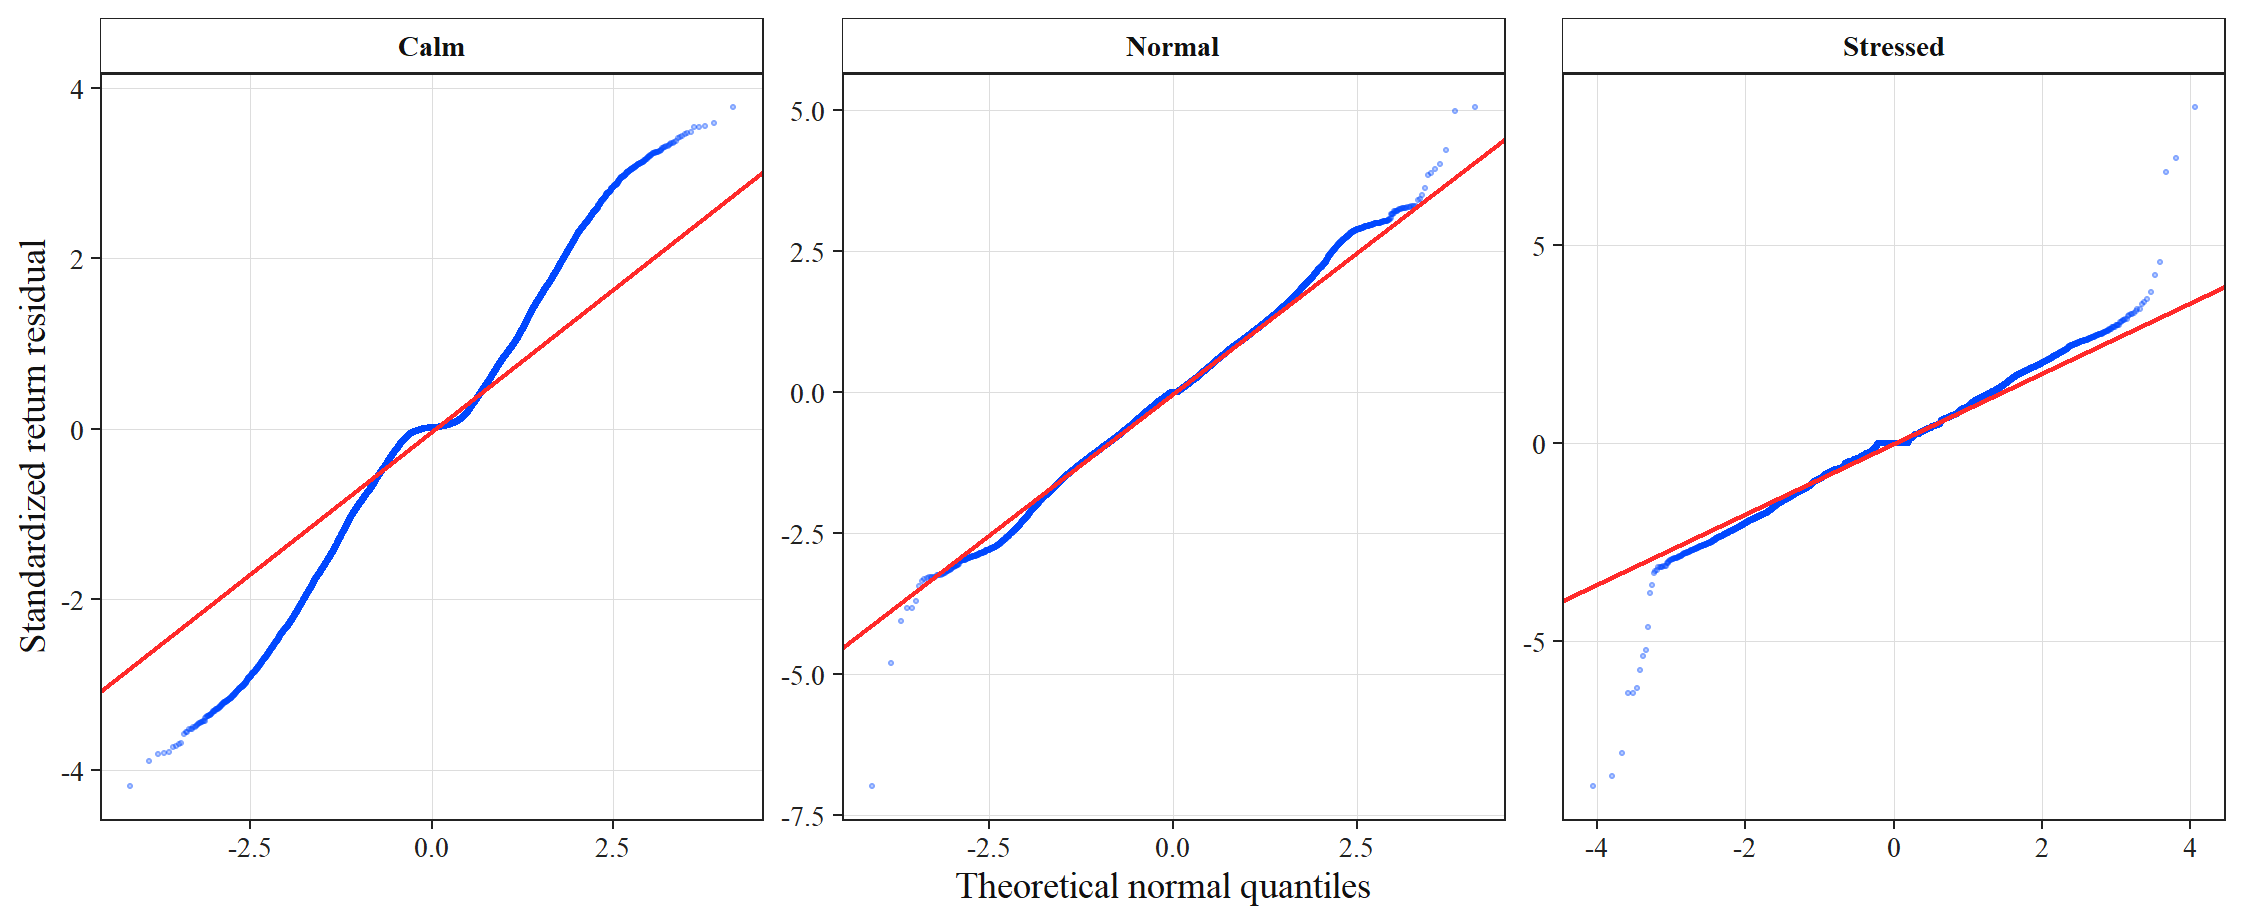
\includegraphics[width=0.82\textwidth]{results/12_hmm_state_interpretation/state_conditional_return_residual_qq.png}
\caption{State-conditional QQ plots for standardized return residuals}
\caption*{\footnotesize\emph{Notes:} The QQ plots are based on standardized residuals from the return emission equation after Viterbi decoding the NHMM state. Normal-state residuals are closest to Gaussian. Calm and Stressed residuals retain visible tail deviations, so the Gaussian model should be read as a transparent classification model rather than a fully specified return distribution.}
\label{fig:qq}
\end{figure}

\figref{fig:qq} shows that state conditioning helps, but does not solve all distributional issues. I keep the Gaussian emission because it gives a transparent and stable state structure. The Student-\(t\) robustness check in \secref{sec:robustness_checks} shows that exact state shares are sensitive to the tail assumption.

A simple pre-HMM price-impact regression also supports the sign convention and the relevance of OFI:
\[
r_t^w=\alpha+\lambda x_t+u_t.
\]
The slope on depth-scaled OFI is positive and statistically significant under ordinary, heteroskedasticity-robust  and day-clustered standard errors (\tabref{tab:price_impact_pre}). The simple regression explains only a small share of return variation  and depth-scaled OFI itself has extremely heavy tails, with kurtosis above 20,000. The HMM therefore uses OFI as a conditioning variable inside state-specific return equations rather than treating it as a Gaussian response.

\begin{table}[!htbp]
\centering
\caption{Pre-HMM price-impact regression}
\small
\begin{tabular}{lrrrr}
\toprule
\textbf{Standard error} & \(\boldsymbol{\hat{\lambda}}\) & \textbf{Std. error} & \(\boldsymbol{t}\)\textbf{-stat.} & \(\boldsymbol{R^2}\) \\
\midrule
OLS & 0.00296 & 0.00003 & 114.34 & 0.0135 \\
HC1 robust & 0.00296 & 0.00043 & 6.86 & 0.0135 \\
Day-clustered HC1 & 0.00296 & 0.00045 & 6.57 & 0.0135 \\
\bottomrule
\end{tabular}
\caption*{\footnotesize\emph{Notes:} The table reports the slope on depth-scaled OFI in \(r_t^w=\alpha+\lambda x_t+u_t\), using 955,110 observations. The point estimate is identical across rows, only the standard error and \(t\)-statistic change with the assumed dependence structure. The coefficient is in return basis points per one unit of raw depth-scaled OFI, not per one-standard-deviation OFI shock.}
\label{tab:price_impact_pre}
\end{table}

\section{Empirical Results}\label{sec:results}

\subsection{Three liquidity-cost regimes}\label{sec:state_results}

\tabref{tab:states} reports the state interpretation. The labels are assigned after estimation by ordering the state spread intercepts from low to high. The Calm state has the lowest spread, highest depth  and strongest price-impact slope. The Normal state has moderate spreads and the highest realized volatility. The Stressed state has the widest spread and lowest depth, but low return volatility and a near-zero price-impact slope.

\begin{table}[htbp]
\centering
\caption{Estimated liquidity-cost regimes}
\small
\begin{tabular}{lrrrrrrrr}
\toprule
\textbf{State} & \textbf{Share} & \(\boldsymbol{\alpha^s}\) & \textbf{Spread} & \textbf{Depth} & \(\boldsymbol{RV}\) & \(\boldsymbol{\lambda}\) & \(\boldsymbol{\sigma_m}\) & \(\boldsymbol{\rho}\) \\
 &  &  & \textbf{bp} &  &  &  &  &  \\
\midrule
Calm & 0.391 & -0.415 & 1.39 & 5,743 & 246 & 43.47 & 1.93 & -0.010 \\
Normal & 0.350 & 0.155 & 2.76 & 4,738 & 669 & 5.79 & 7.27 & 0.003 \\
Stressed & 0.260 & 0.417 & 3.52 & 4,381 & 251 & 0.12 & 2.51 & 0.003 \\
\bottomrule
\end{tabular}
\caption*{\footnotesize\emph{Notes:} \(\alpha^s\) is the state intercept of the de-seasonalized log relative spread and is used to order states from low to high spread. \(\lambda\) is the coefficient on depth-scaled OFI after scaling by the full-sample standard deviation of that flow variable. It is measured in basis points per one-standard-deviation OFI shock. \(RV\) is the state-weighted mean backward-looking six-minute realized variance. State shares are posterior shares from the NHMM.}
\label{tab:states}
\end{table}

The key interpretation is that Stressed is a liquidity-withdrawal state. It is stressed in the order book, not mainly in realized volatility. Spreads are wide and depth is low, but price changes are muted and order flow no longer maps strongly into returns. The label should still be read as model-based: Stressed has the heaviest return residual tails, so large individual return shocks do occur inside this state. The regime is more naturally read as liquidity withdrawal than continuous panic selling.

One caution is needed for \(\lambda_i\), the state-specific price-impact slope. It measures the return response to scaled OFI inside each state, but it also depends on how cleanly scaled OFI works as an explanatory variable in that state. In Calm, depth is high and stable, so depth-scaled OFI is measured more smoothly. In Stressed, depth is lower and changes more sharply, so the fitted slope can be pushed toward zero even if trading conditions are still poor. This does not overturn the main interpretation, because the same high-spread state also appears in the 5-second trade-bucket, signed-volume  and 60-second robustness checks. Still, the Calm-to-Stressed slope gap should be read as a large point-estimate difference, not as an exact structural multiple.

\begin{figure}[!htbp]
\centering
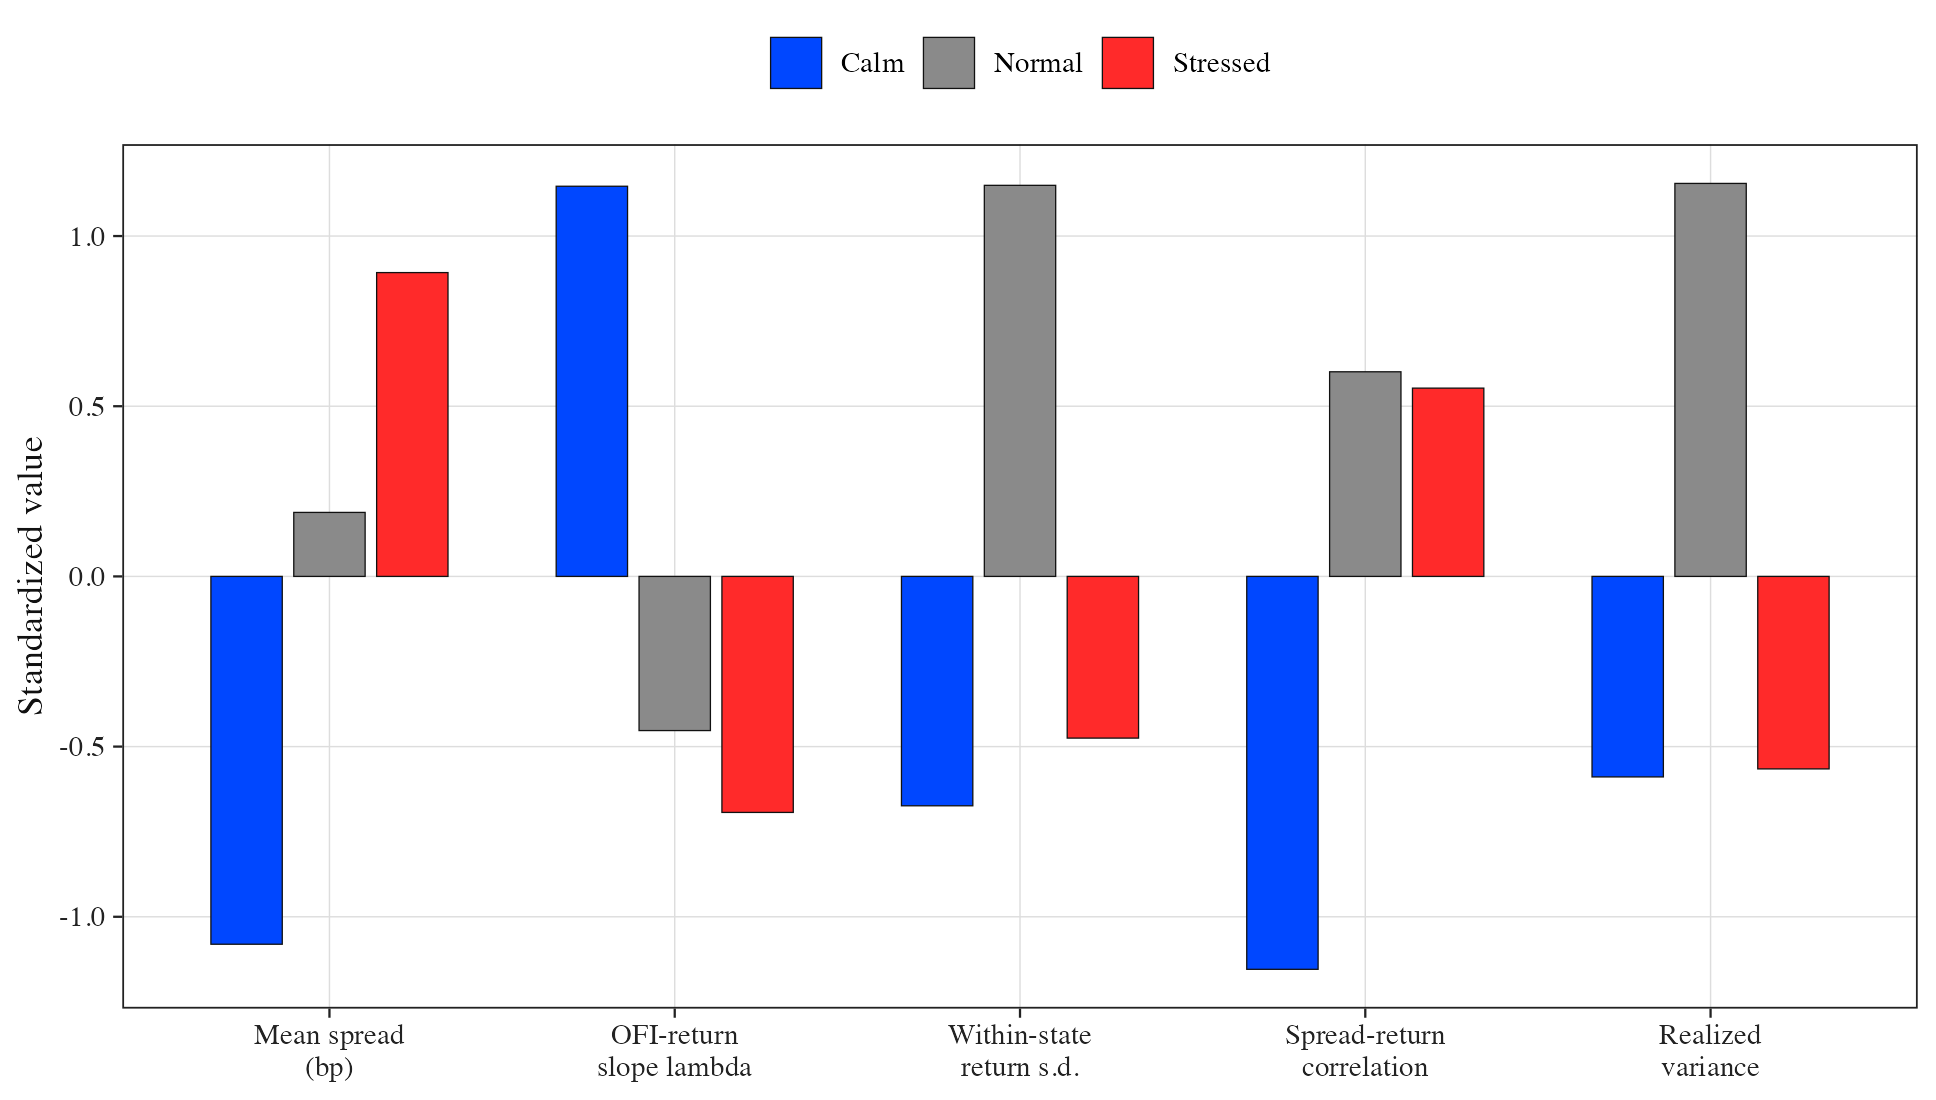
\includegraphics[width=0.76\textwidth]{results/12_hmm_state_interpretation/state_interpretation.png}
\caption{State interpretation: relative position of spreads, price impact, volatility  and covariance}
\caption*{\footnotesize\emph{Notes:} The figure standardizes each metric across states, so the bars show relative rather than raw magnitudes. Calm has the strongest OFI-return slope, Normal has the highest realized and within-state return volatility  and Stressed has the widest spread.}
\label{fig:state_interpretation}
\end{figure}

\subsection{Regime persistence and classification}\label{sec:persistence_classification}

The constant-transition matrix in \tabref{tab:constant_transition} shows that states are persistent but short-lived. Expected dwell times are 1.40 minutes for Calm, 2.15 minutes for Normal  and 1.12 minutes for Stressed. These are minute-scale episodes, not daily or weekly market phases.

\begin{table}[!htbp]
\centering
\caption{Constant-transition HMM: transition matrix}
\small
\begin{tabular}{lccc}
\toprule
\textbf{Current state} & \textbf{Calm} & \textbf{Normal} & \textbf{Stressed} \\
\midrule
Calm & 0.644 & 0.148 & 0.208 \\
Normal & 0.138 & 0.767 & 0.095 \\
Stressed & 0.349 & 0.096 & 0.555 \\
\bottomrule
\end{tabular}
\caption*{\footnotesize\emph{Notes:} Rows sum to one. The model is estimated on 30-second stock-day sequences.}
\label{tab:constant_transition}
\end{table}

Classification uncertainty is moderate. A smoothed posterior probability is the model's probability that a bucket belongs to a given state after using information from the whole stock-day sequence. The maximum smoothed posterior is the model's confidence in its most likely state for that bucket. The average maximum value is 0.879. About 15.1\% of observations have maximum posterior below 0.70  and 24.6\% have maximum posterior below 0.80. Roughly one in four buckets is therefore somewhat ambiguous between states. Decoded paths should be interpreted as useful summaries of posterior probabilities, not as perfectly observed regimes. \figref{fig:liquidity_panel} shows a representative stock-day panel with posterior state probabilities, transformed spread  and rolling price impact.

\begin{figure}[!htbp]
\centering
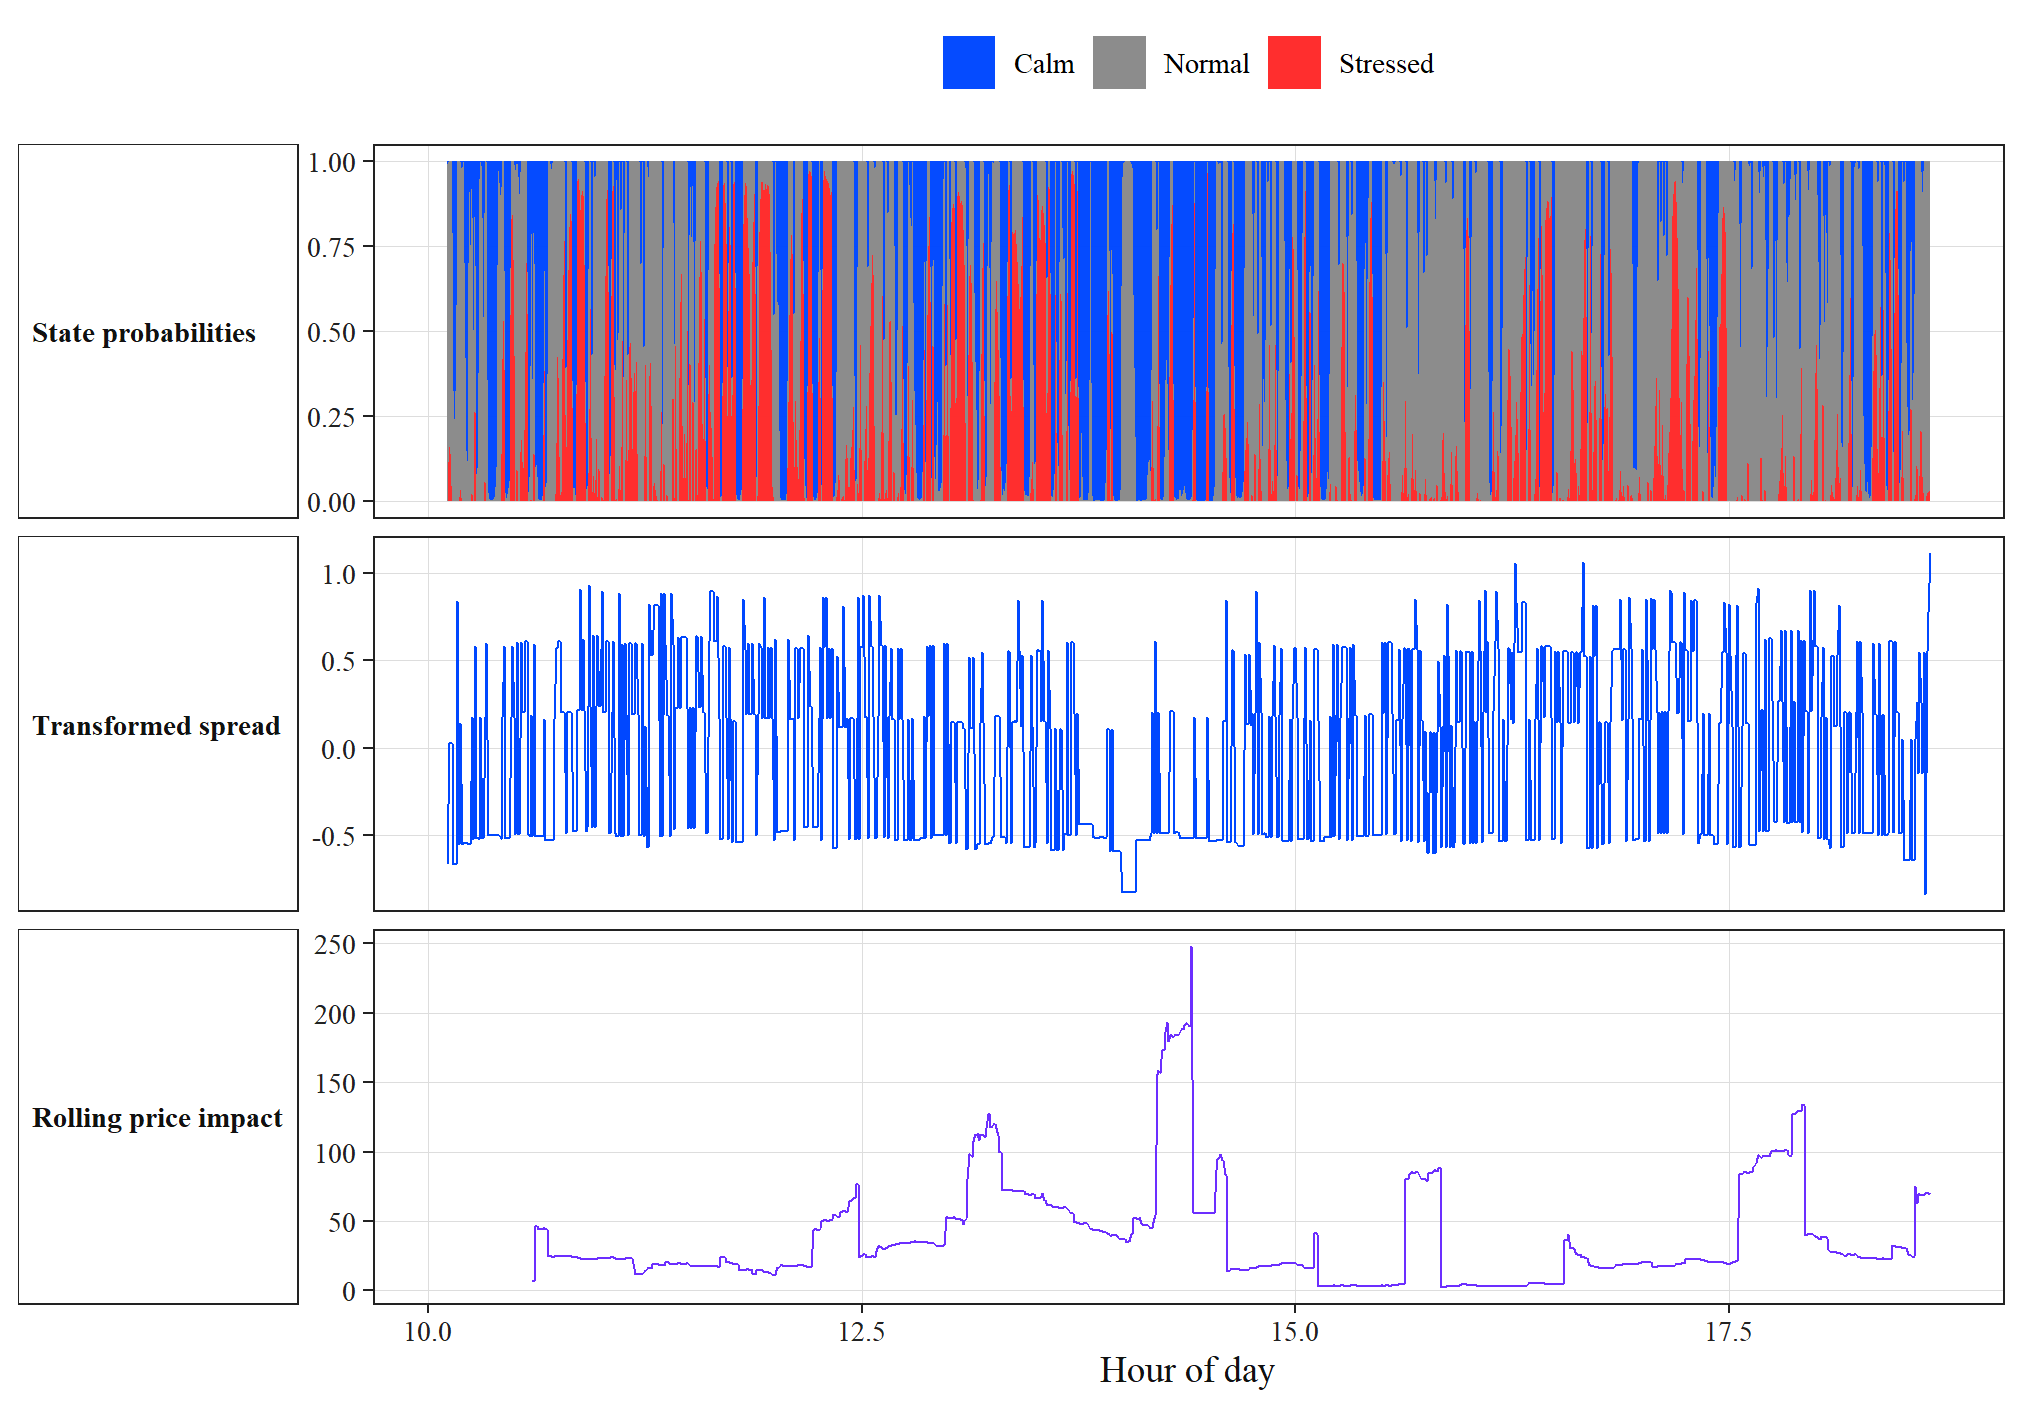
\includegraphics[width=0.86\textwidth]{results/08_hmm_state_probabilities/nhmm_probability_liquidity_panel.png}
\caption{Regime probabilities and liquidity variables on a representative stock-day}
\caption*{\footnotesize\emph{Notes:} The top panel stacks smoothed probabilities of Calm, Normal  and Stressed states. The lower panels show transformed spread and a rolling price-impact estimate. The bottom panel is a right-aligned 60-bucket or 30-minute, no-intercept OLS slope of \(r_t^w\) on scaled depth-adjusted OFI, measured in basis points per one-standard-deviation OFI shock. The plot illustrates that state changes are short-lived and often align with changes in quoted liquidity and local price sensitivity.}
\label{fig:liquidity_panel}
\end{figure}

\figref{fig:intraday_profile} reports the mean smoothed probability of the Stressed state by time of day. The probability is nearly flat across the day at roughly 25\%, with a small opening dip and little end-of-day spike. This differs from the classic U-shape of raw spreads and fits the variable construction: deterministic open/close widening has already been removed from the level variables seen by the HMM.

\begin{figure}[!htbp]
\centering
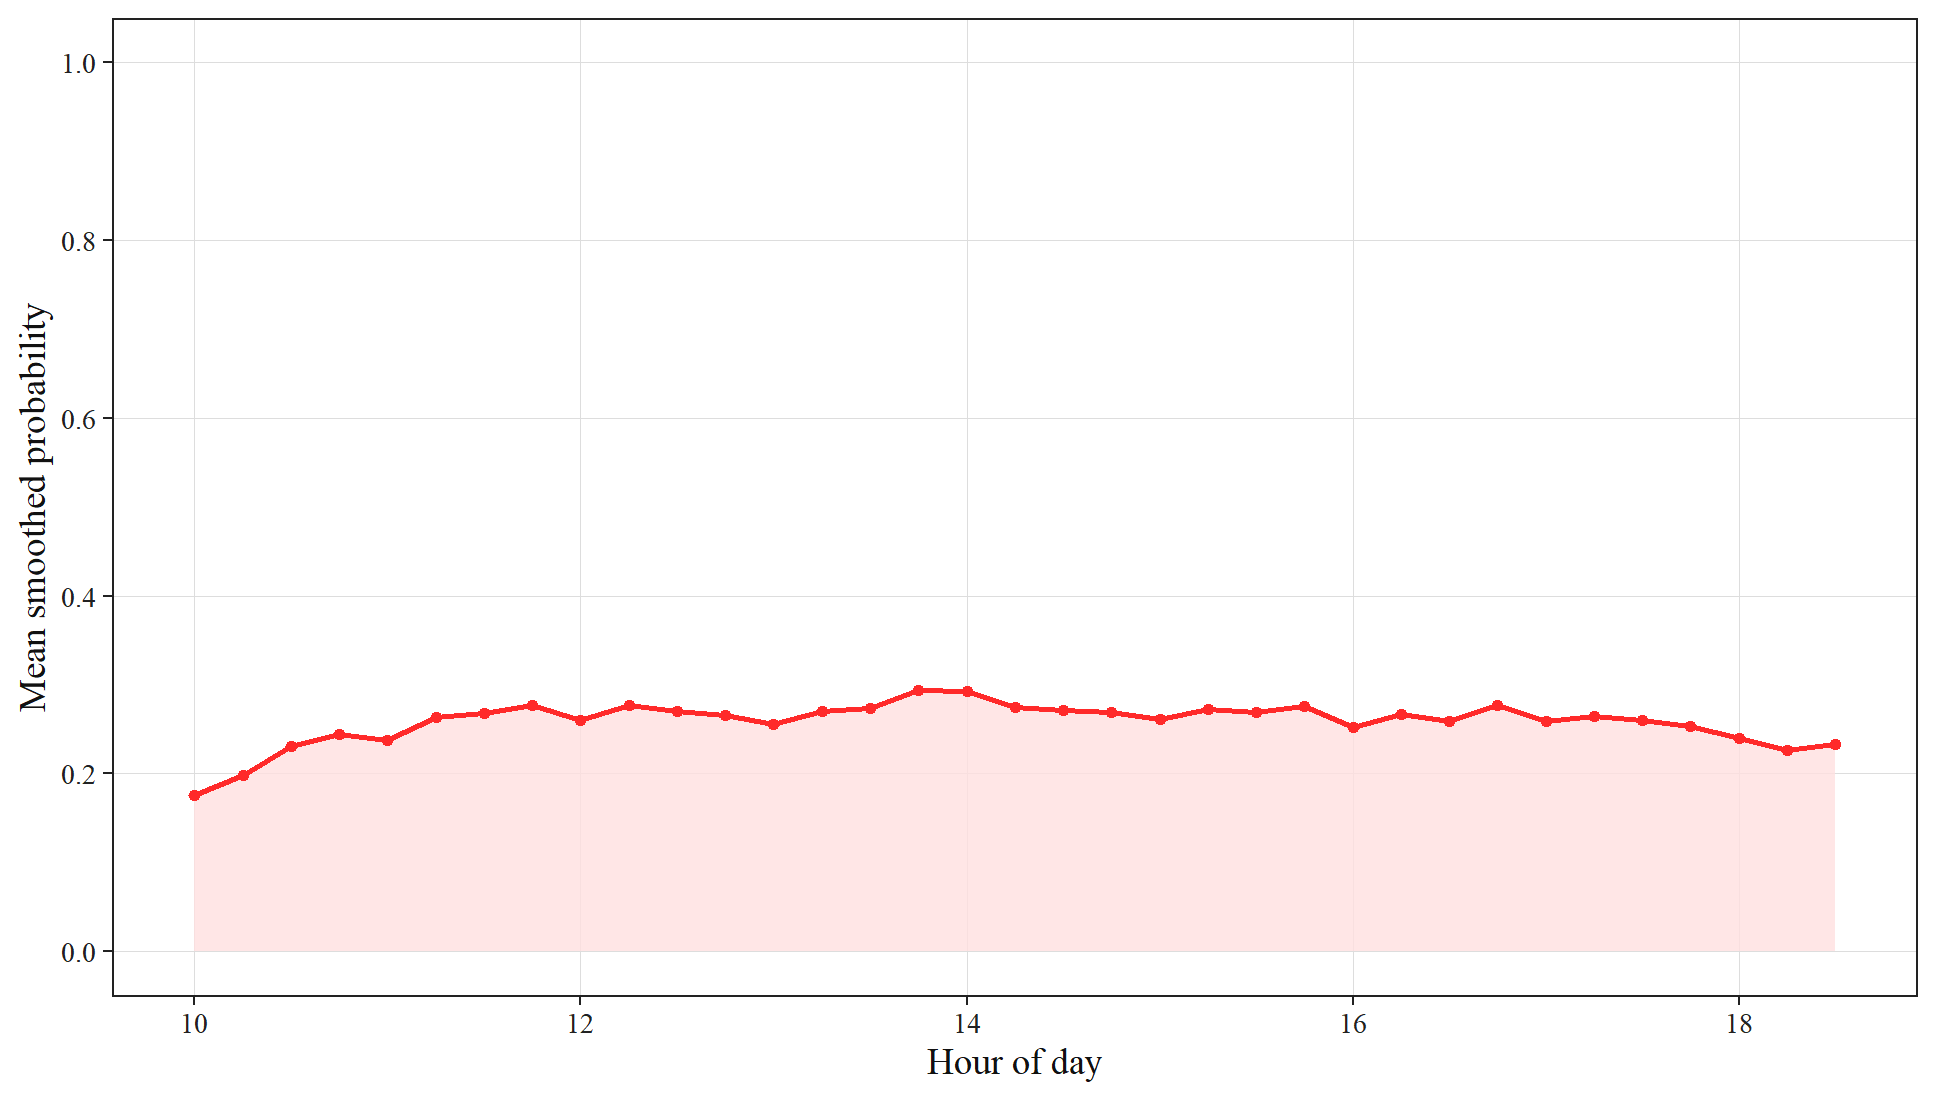
\includegraphics[width=0.74\textwidth]{results/08_hmm_state_probabilities/stressed_probability_intraday_profile.png}
\caption{Mean intraday probability of the Stressed liquidity-withdrawal regime}
\caption*{\footnotesize\emph{Notes:} Smoothed posterior probabilities are averaged over stocks and days in 15-minute bins. The figure is descriptive and uses the completed sample, so it should not be read as a real-time filtered probability.}
\label{fig:intraday_profile}
\end{figure}

\subsection{Covariate-driven transitions}\label{sec:transition_results}

The covariate-transition HMM improves the fit. \tabref{tab:model_comparison} compares three models on the same 30-second primary sample. Moving from a one-state Gaussian conditional model to a three-state HMM reduces BIC by more than one million points. Allowing transitions to depend on market conditions further reduces BIC by 38,023 points relative to the constant-transition HMM. Per observation, this is about 0.04 BIC units, so the improvement is modest but consistent given the large sample.

\begin{table}[!htbp]
\centering
\caption{Model comparison on the primary 30-second sample}
\small
\begin{tabular}{lrrrr}
\toprule
\textbf{Model} & \textbf{logLik} & \textbf{Parameters} & \textbf{BIC} & \(\boldsymbol{\Delta}\)\textbf{BIC} \\
\midrule
3-state NHMM, covariate transitions & -3,074,937 & 54 & 6,150,618 & 0 \\
3-state HMM, constant transitions & -3,094,155 & 24 & 6,188,641 & 38,023 \\
1-state Gaussian conditional model & -3,618,941 & 6 & 7,237,965 & 1,087,346 \\
\bottomrule
\end{tabular}
\caption*{\footnotesize\emph{Notes:} All three models use the same observations and the same response and flow variables. \(\Delta\)BIC is relative to the best model.}
\label{tab:model_comparison}
\end{table}

The average transition matrix implied by the NHMM is shown in \tabref{tab:nhmm_transition}. Compared with the constant-transition model, average persistence is lower because the transition probabilities now vary with market conditions. The Stressed state still has a meaningful recovery channel directly to Calm.

\begin{table}[!htbp]
\centering
\caption{NHMM average implied transition matrix}
\small
\begin{tabular}{lccc}
\toprule
\textbf{Current state} & \textbf{Calm} & \textbf{Normal} & \textbf{Stressed} \\
\midrule
Calm & 0.579 & 0.216 & 0.205 \\
Normal & 0.181 & 0.682 & 0.136 \\
Stressed & 0.323 & 0.153 & 0.524 \\
\bottomrule
\end{tabular}
\caption*{\footnotesize\emph{Notes:} Entries are transition probabilities averaged over the observed covariate distribution.}
\label{tab:nhmm_transition}
\end{table}

Average marginal effects are easier to interpret than raw multinomial-logit coefficients. An average marginal effect asks: if one covariate changes while the observed rows are otherwise kept as they are, how much does the transition probability change on average? \tabref{tab:ame} and \figref{fig:ame} show the effect of a one-unit increase in each covariate on two probabilities: entry from Calm to Stressed and exit from Stressed to Calm.

\begin{table}[!htbp]
\centering
\caption{Average marginal effects on Stressed-state entry and recovery}
\scriptsize
\setlength{\tabcolsep}{3pt}
\begin{tabular}{@{}lrrrrl@{}}
\toprule
\textbf{Covariate} & \textbf{Entry AME} & \textbf{95\% CI} & \textbf{Exit AME} & \textbf{95\% CI} & \textbf{Direction} \\
\midrule
Depth \(\tilde{D}_t\) & -0.050 & [-0.053, -0.048] & 0.042 & [0.039, 0.046] & H1 \\
Realized volatility & -0.020 & [-0.026, -0.014] & -0.053 & [-0.062, -0.044] & mixed \\
Absolute OFI pressure & -0.001 & [-0.006, 0.003] & -0.034 & [-0.050, -0.022] & H2b \\
Open dummy & -0.035 & [-0.055, -0.017] & -0.002 & [-0.024, 0.024] & H3 \\
Close dummy & -0.022 & [-0.034, -0.011] & -0.025 & [-0.043, -0.006] & H3 \\
\bottomrule
\end{tabular}
\caption*{\footnotesize\emph{Notes:} Entry is the change in the probability of moving from Calm to Stressed in the next bucket. Exit is the change in the probability of moving from Stressed to Calm. For continuous variables, the AME is the average effect of a one-unit increase. For the open and close dummies, it is the change from 0 to 1. Confidence intervals are from 200 day-cluster bootstrap replications.}
\label{tab:ame}
\end{table}

\begin{figure}[!htbp]
\centering
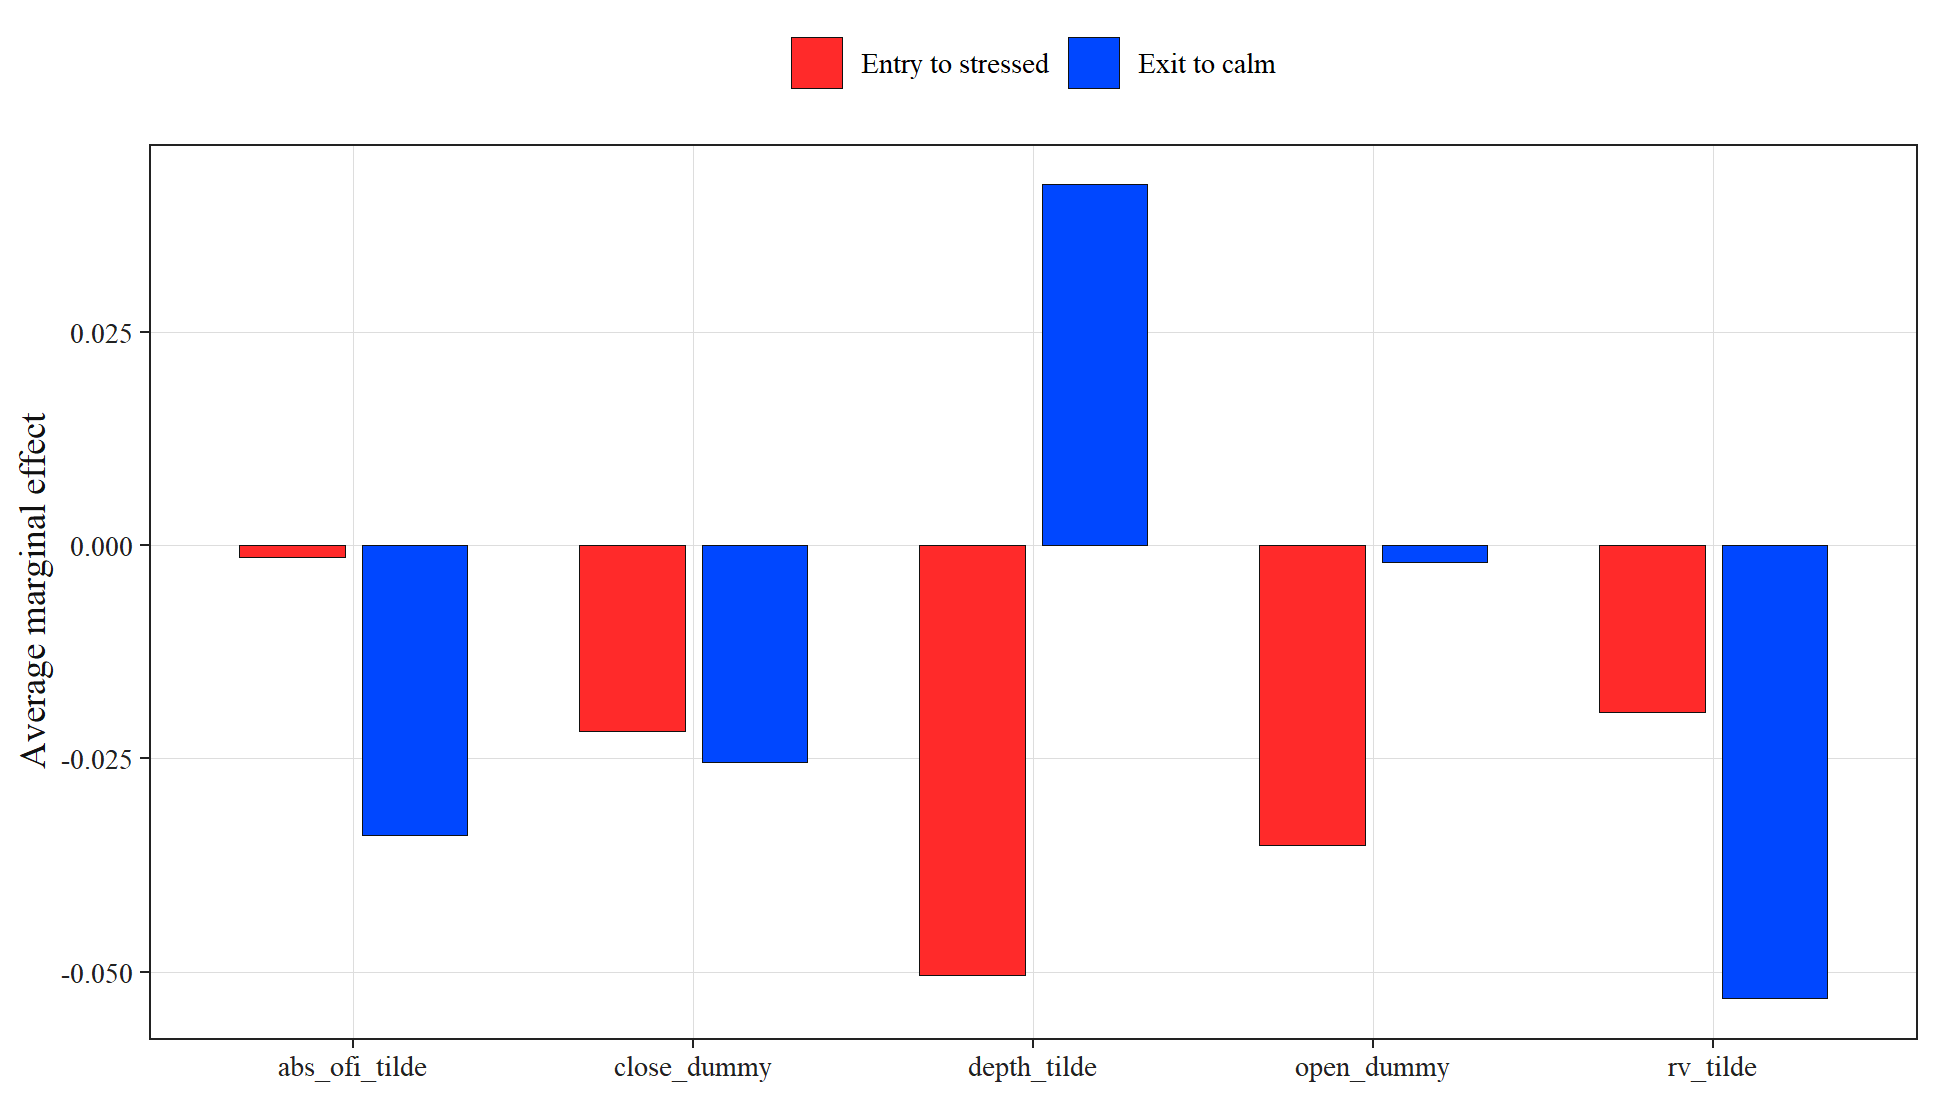
\includegraphics[width=0.78\textwidth]{results/10_hmm_covariate_transition/transition_average_marginal_effects.png}
\caption{Average marginal effects for entry into and exit from the Stressed state}
\caption*{\footnotesize\emph{Notes:} Red bars show how each variable changes the chance of moving from Calm to Stressed. Blue bars show how each variable changes the chance of moving from Stressed back to Calm. The most important pattern is depth: thin books predict entry into Stressed, while deeper books predict recovery.}
\label{fig:ame}
\end{figure}

The depth result supports the main fragility mechanism. A one-unit increase in de-seasonalized depth is associated with a 5.0 percentage point lower probability of Calm-to-Stressed entry and a 4.2 percentage point higher probability of Stressed-to-Calm recovery. Among the five covariates, depth has the largest and most stable transition effect in the reported AMEs.

The volatility and OFI effects are more nuanced. Higher realized volatility predicts both lower entry into Stressed from Calm and lower recovery from Stressed to Calm. The first sign supports the idea that Stressed is not mainly a high-volatility entry state. The second is harder to interpret: it may route the market toward Normal or it may make Stressed more persistent once entered. Absolute OFI pressure does not significantly trigger Stressed entry, but it significantly reduces recovery. This suggests that OFI pressure is more of a propagation mechanism than an ignition mechanism for liquidity withdrawal: it keeps stress from clearing, rather than clearly starting it.

The transition equation should be read as reduced-form. Depth, volatility  and OFI pressure are all market outcomes as well as predictors. The estimates therefore describe which observed conditions precede state changes. They do not prove that changing depth alone would causally move the market between regimes.

\section{Robustness and Limitations}\label{sec:robustness}

\subsection{Robustness checks}\label{sec:robustness_checks}

The robustness script estimates five constant-transition HMM variants. These checks target the state model rather than the NHMM transition equation. They ask whether the three-state structure, the OFI flow variable  and the 30-second frequency are essential for the main interpretation.

\begin{table}[!htbp]
\centering
\caption{Robustness checks}
\scriptsize
\setlength{\tabcolsep}{3pt}
\begin{tabularx}{\textwidth}{L{0.25\textwidth}C{0.11\textwidth}C{0.15\textwidth}X}
\toprule
\textbf{Specification} & \textbf{Converged} & \textbf{State shares} & \textbf{Interpretation} \\
\midrule
2-state Gaussian, same emissions & Yes & 0.379 / 0.621 & Two states are too coarse, the three-state structure separates active trading from liquidity withdrawal. \\
Student-\(t\), \(\nu=5\) & No, maxit & 0.121 / 0.389 / 0.489 & Heavy-tail emissions reshape state shares and need more work, result is a sensitivity check, not a clean confirmation. \\
5-second trade buckets & Yes & 0.410 / 0.420 / 0.170 & Three regimes survive at higher frequency, but trade-bucket sampling misses no-trade liquidity-withdrawal periods. \\
Signed-volume flow instead of OFI & Yes & 0.414 / 0.297 / 0.289 & The state structure survives, but the fit is worse than the OFI-based primary specification on the same sample. \\
60-second frequency & Yes & 0.406 / 0.305 / 0.289 & The regime structure is similar, supporting 30 seconds as a reasonable primary frequency. \\
\bottomrule
\end{tabularx}
\caption*{\footnotesize\emph{Notes:} The table asks whether the main state interpretation survives reasonable changes in the model. BIC values are not compared across different sampling frequencies because the observation counts differ. The signed-volume and two-state checks are directly comparable to the primary constant-transition specification because they use the same 30-second sample.}
\label{tab:robustness}
\end{table}

The robustness checks are not uniform, but they support the main three-state interpretation. The three-state structure is identified, OFI is preferred to signed volume in the HMM  and the result is not an artifact of choosing exactly 30 seconds. The Student-\(t\) check is the main unresolved point. It did not converge in 50 EM iterations and allocates 48.9\% of observations to the high-spread state, compared with 26.0\% under the Gaussian primary model. This is the largest robustness disagreement. I therefore emphasize the qualitative structure -- low-spread Calm, active Normal  and high-spread Stressed -- more than the exact Stressed-state share.

\subsection{Limitations}\label{sec:limitations}

Several limitations matter. First, the estimates are reduced-form: depth, volatility  and order-flow pressure are jointly determined with hidden liquidity states, so the transition effects are predictive associations rather than causal estimates. In other words, the model shows which conditions tend to come before state changes, but it does not prove what would happen if depth could be changed experimentally.

Second, the pooled model constrains emissions and transition dynamics to be common across 15 heterogeneous stocks. The decoded Stressed share varies from about 20\% for GAZP to about 41\% for HEAD (\apptabref{tab:per_stock}). Across stocks, those that spend more time in Stressed also tend to have a wider mean spread conditional on being Stressed (\appfigref{fig:per_stock_scatter}). The pooled HMM cannot exploit this cross-sectional pattern, which is another reason a per-stock or hierarchical specification is the natural next step.

Third, the model uses best-level OFI rather than multi-level order-book imbalance or cross-stock OFI. Multi-level OFI \citep{XuGouldHowison2019} and cross-impact measures \citep{ContCucuringuZhang2023} would be natural extensions, especially in a pooled blue-chip panel. Finally, trade-sign and OFI reconstruction are necessarily imperfect because exchange order-log conventions require careful interpretation of repeated trade rows and resting-side indicators. The sample covers one three-month period in 2025 and does not explicitly adjust for corporate actions, trading halts or special events beyond the cleaning rules embedded in the reconstructed top-of-book sample.

\section{Conclusion}\label{sec:conclusion}

This paper builds an empirical workflow for intraday liquidity-cost states in the MOEX limit order book. The reason for doing this is not only to classify observations. It is to show that the same market can move through different short-lived liquidity-cost regimes and that an average price-impact estimate hides this movement. The code reconstructs best quotes from event-level order logs, builds 30-second stock-day sequences, constructs OFI and de-seasonalized liquidity variables, estimates a three-state HMM  and then allows transition probabilities to depend on observable order-book conditions.

The main finding is that price impact is strongly state-dependent. Calm has tight spreads, deep books  and a strong OFI-return relation. Normal is the active price-discovery state, with the highest return volatility. Stressed has the widest spreads and thinnest book, but a near-zero price-impact slope and relatively low realized volatility. I interpret it as liquidity withdrawal rather than continuous panic selling.

The transition results support a depth-fragility mechanism. Low depth predicts entry into the Stressed state  and higher depth predicts recovery. This is the main value added by the NHMM: it links the hidden liquidity state to observable conditions in the book instead of only reporting average regime persistence. Realized volatility and absolute OFI pressure mainly affect persistence and routing. The results should be read as reduced-form evidence: they show that observable order-book conditions help identify short-lived liquidity-cost states, but they do not establish a structural causal effect of depth or order flow. The sample period also makes this one of the first intraday liquidity-regime studies of MOEX after the structural change in the Russian equity market that began in 2022, which limits the available comparison set for the depth-fragility result. Future work could estimate stock-specific or hierarchical state dynamics, use multi-level order-book imbalance  and revisit the heavy-tail emission with a fully converged Student-\(t\) or mixture specification.

\clearpage
\phantomsection
\section*{Appendix}\label{sec:appendix}
\addcontentsline{toc}{section}{Appendix}

\begin{table}[htbp]
\centering
\caption{Per-stock Stressed-state shares}
\scriptsize
\setlength{\tabcolsep}{4pt}
\begin{tabular}{lrrrr}
\toprule
\textbf{Stock} & \textbf{Share} & \textbf{Spread bp} & \textbf{Depth} & \textbf{Avg. max post.} \\
 &  & \textbf{(Stressed)} & \textbf{(Stressed)} &  \\
\midrule
HEAD & 0.407 & 7.67 & 227 & 0.900 \\
SNGS & 0.347 & 5.79 & 34,816 & 0.873 \\
PLZL & 0.338 & 3.07 & 306 & 0.860 \\
TATN & 0.307 & 3.30 & 786 & 0.890 \\
YDEX & 0.306 & 3.20 & 204 & 0.883 \\
T & 0.301 & 1.61 & 283 & 0.894 \\
LKOH & 0.280 & 1.84 & 170 & 0.900 \\
NLMK & 0.277 & 3.77 & 3,647 & 0.879 \\
CHMF & 0.260 & 4.54 & 558 & 0.890 \\
SBER & 0.246 & 0.97 & 4,339 & 0.866 \\
ROSN & 0.245 & 2.48 & 1,150 & 0.885 \\
GMKN & 0.220 & 3.88 & 6,056 & 0.862 \\
MOEX & 0.215 & 1.99 & 1,537 & 0.858 \\
NVTK & 0.210 & 3.86 & 717 & 0.867 \\
GAZP & 0.197 & 1.86 & 5,660 & 0.884 \\
\bottomrule
\end{tabular}
\caption*{\footnotesize\emph{Notes:} The share is the fraction of a stock's observations decoded as Stressed. Spread and depth are averaged only over observations decoded as Stressed, so they describe what Stressed looks like for each stock. The \(\lambda\) coefficients are not shown by stock because the primary model estimates one pooled set of state slopes for all 15 stocks.}
\label{tab:per_stock}
\end{table}

\begin{figure}[!htbp]
\centering
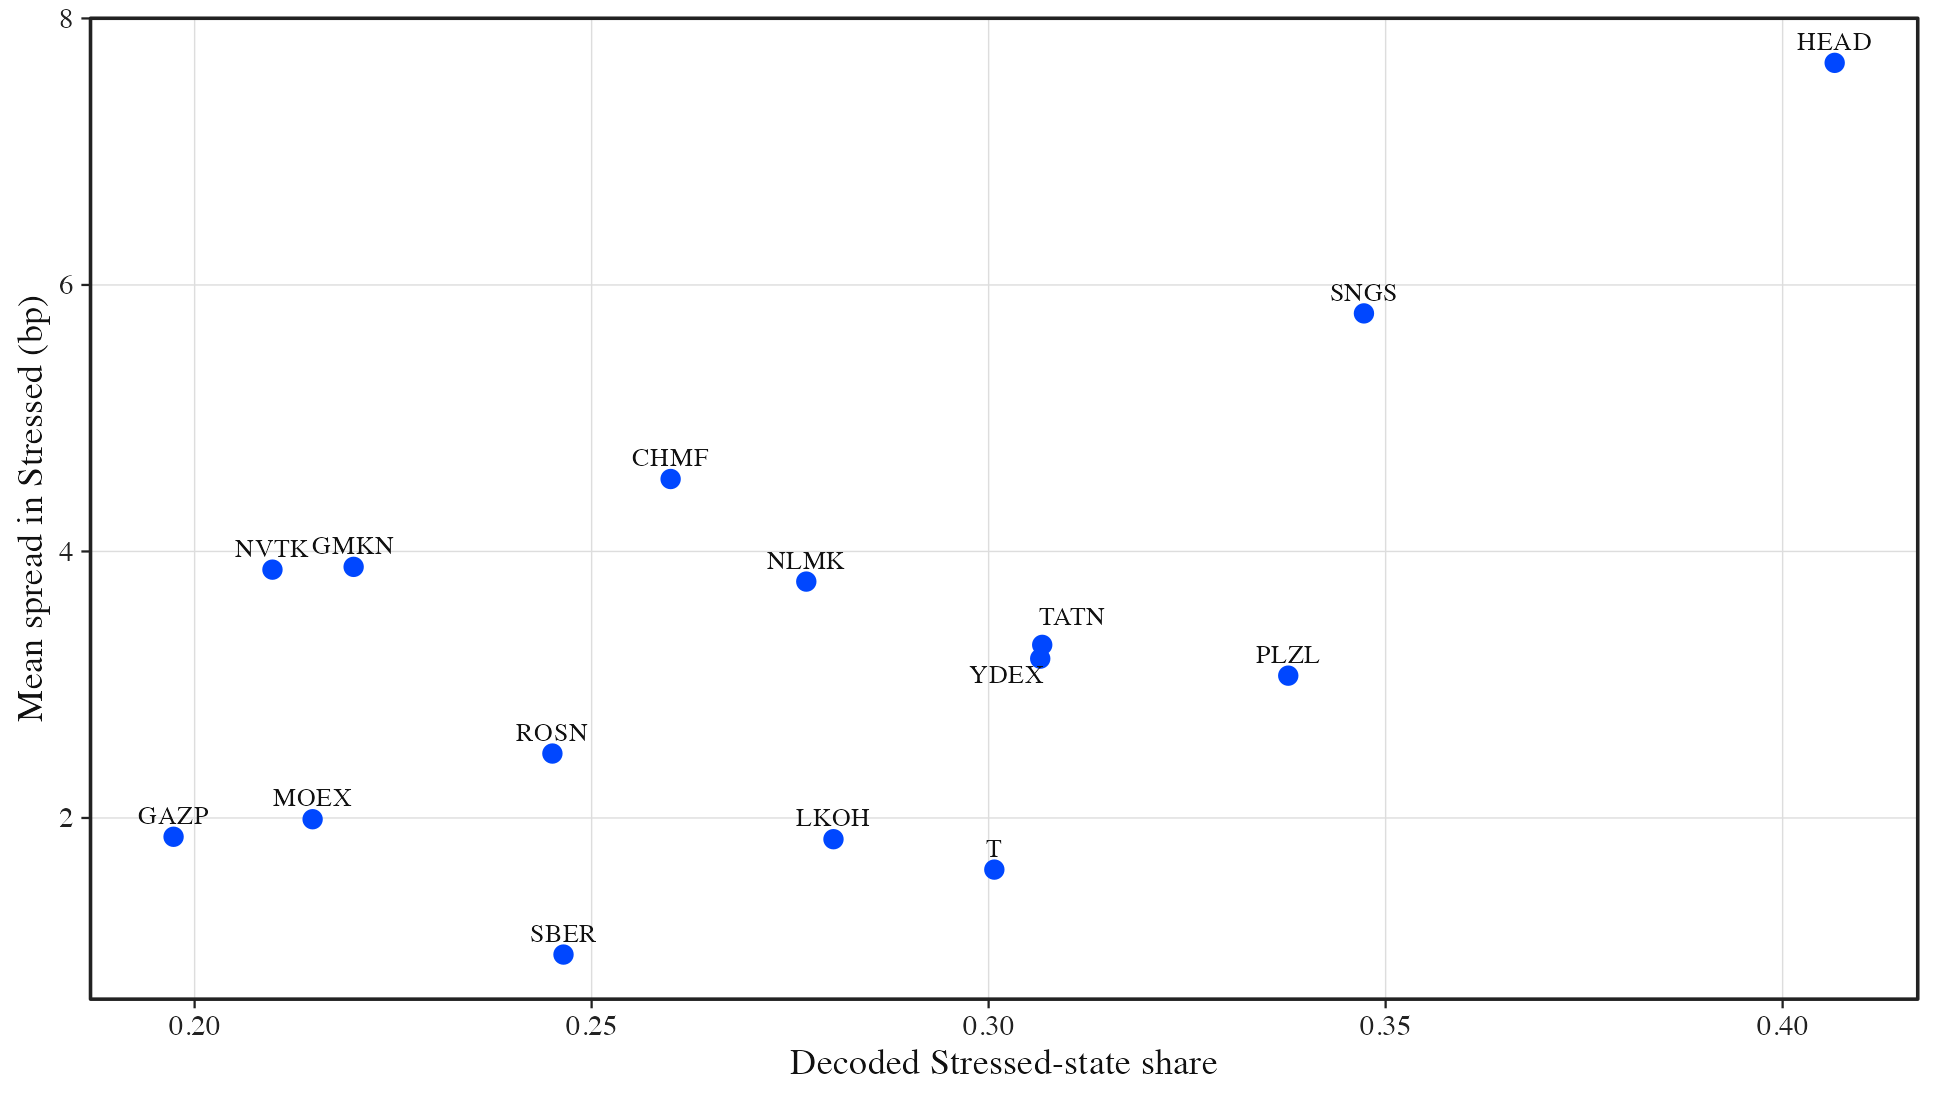
\includegraphics[width=0.78\textwidth]{results/15_hmm_state_sequence_diagnostics/per_stock_stressed_share_spread.png}
\caption{Per-stock Stressed-state share and Stressed-state spread}
\caption*{\footnotesize\emph{Notes:} Each point is one stock. The horizontal axis shows how often the stock is decoded as Stressed; the vertical axis shows its average spread during those Stressed buckets. The upward pattern means that stocks spending more time in Stressed also tend to have more expensive trading conditions when Stressed.}
\label{fig:per_stock_scatter}
\end{figure}

\begin{table}[htbp]
\centering
\caption{State-conditional residual kurtosis}
\small
\begin{tabular}{lrrr}
\toprule
\textbf{State} & \textbf{Return kurtosis} & \textbf{Spread kurtosis} & \textbf{Observations} \\
\midrule
Calm & 4.22 & 2.34 & 390,993 \\
Normal & 3.56 & 2.22 & 299,454 \\
Stressed & 4.58 & 3.20 & 264,663 \\
\bottomrule
\end{tabular}
\caption*{\footnotesize\emph{Notes:} Kurtosis measures tail thickness. A normal distribution has kurtosis 3, so values above 3 mean heavier tails than normal. The return residuals therefore still have moderate tail excess after state conditioning, especially in Calm and Stressed.}
\label{tab:residual_kurtosis}
\end{table}

\begin{table}[htbp]
\centering
\caption{Baseline HMM convergence across starting values}
\small
\begin{tabular}{crrr}
\toprule
\textbf{Start} & \textbf{Log-likelihood} & \textbf{Iterations} & \textbf{Convergence code} \\
\midrule
1 & -3,094,155.40 & 71 & 0 \\
2 & -3,094,155.54 & 71 & 0 \\
3 & -3,094,155.33 & 71 & 0 \\
4 & -3,094,155.44 & 71 & 0 \\
\bottomrule
\end{tabular}
\caption*{\footnotesize\emph{Notes:} Each row starts the EM algorithm from a different initial guess. The final log-likelihoods are almost identical, which means the baseline HMM solution is not driven by one lucky starting value. States are relabelled after estimation by ascending spread intercept.}
\label{tab:starts}
\end{table}

\FloatBarrier

\begin{figure}[!htbp]
\centering
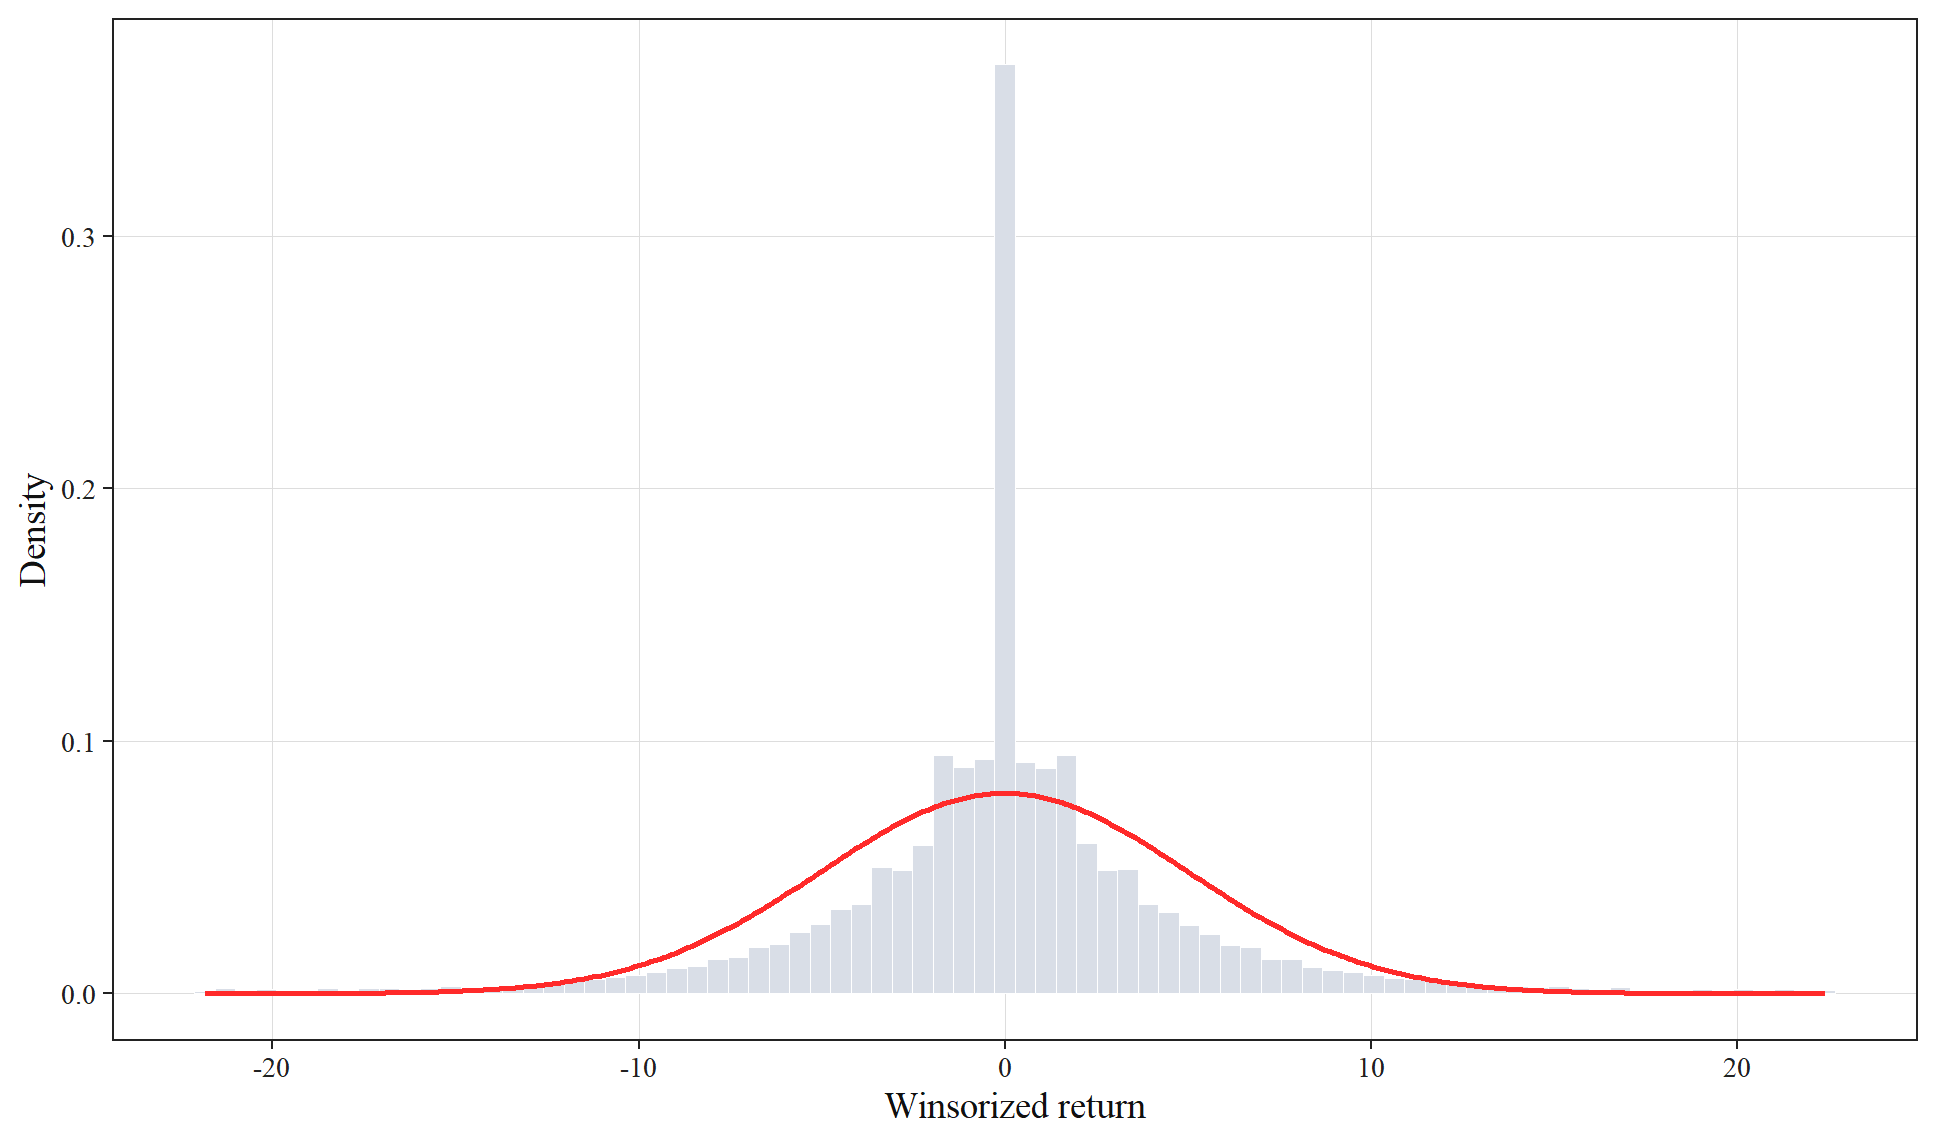
\includegraphics[width=0.78\textwidth]{results/04_normality/hist_r_t_winsorized_normal_overlay.png}
\caption{Winsorized returns and normal overlay}
\caption*{\footnotesize\emph{Notes:} The tall central spike means many 30-second buckets still have exactly zero return. This explains why the Gaussian emission is used as a practical classification approximation, not as a literal claim that all intraday returns are normally distributed.}
\label{fig:appendix_normality}
\end{figure}

\begin{figure}[!htbp]
\centering
\begin{subfigure}{0.48\textwidth}
\centering
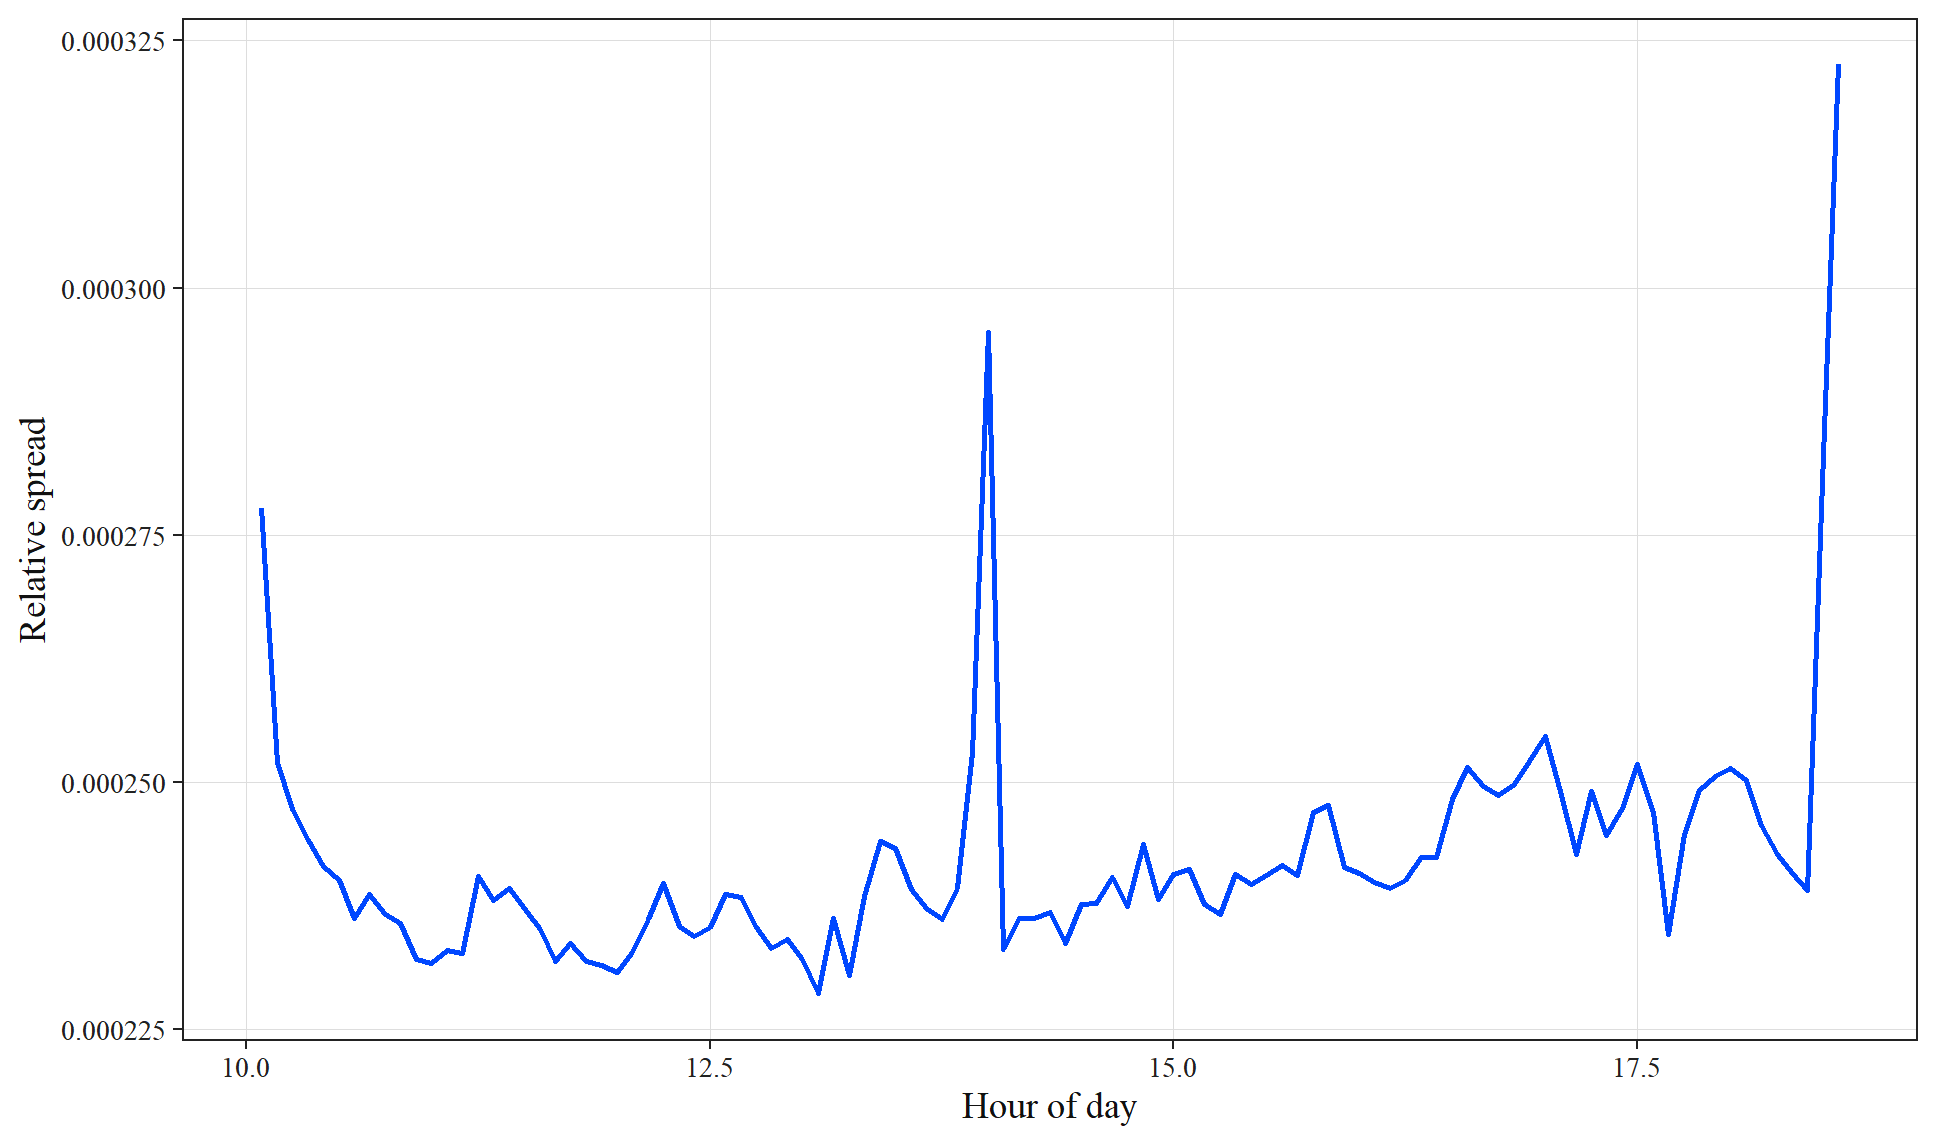
\includegraphics[width=\textwidth]{results/02_seasonality/intraday_relative_spread.png}
\caption{Relative spread}
\end{subfigure}
\hfill
\begin{subfigure}{0.48\textwidth}
\centering
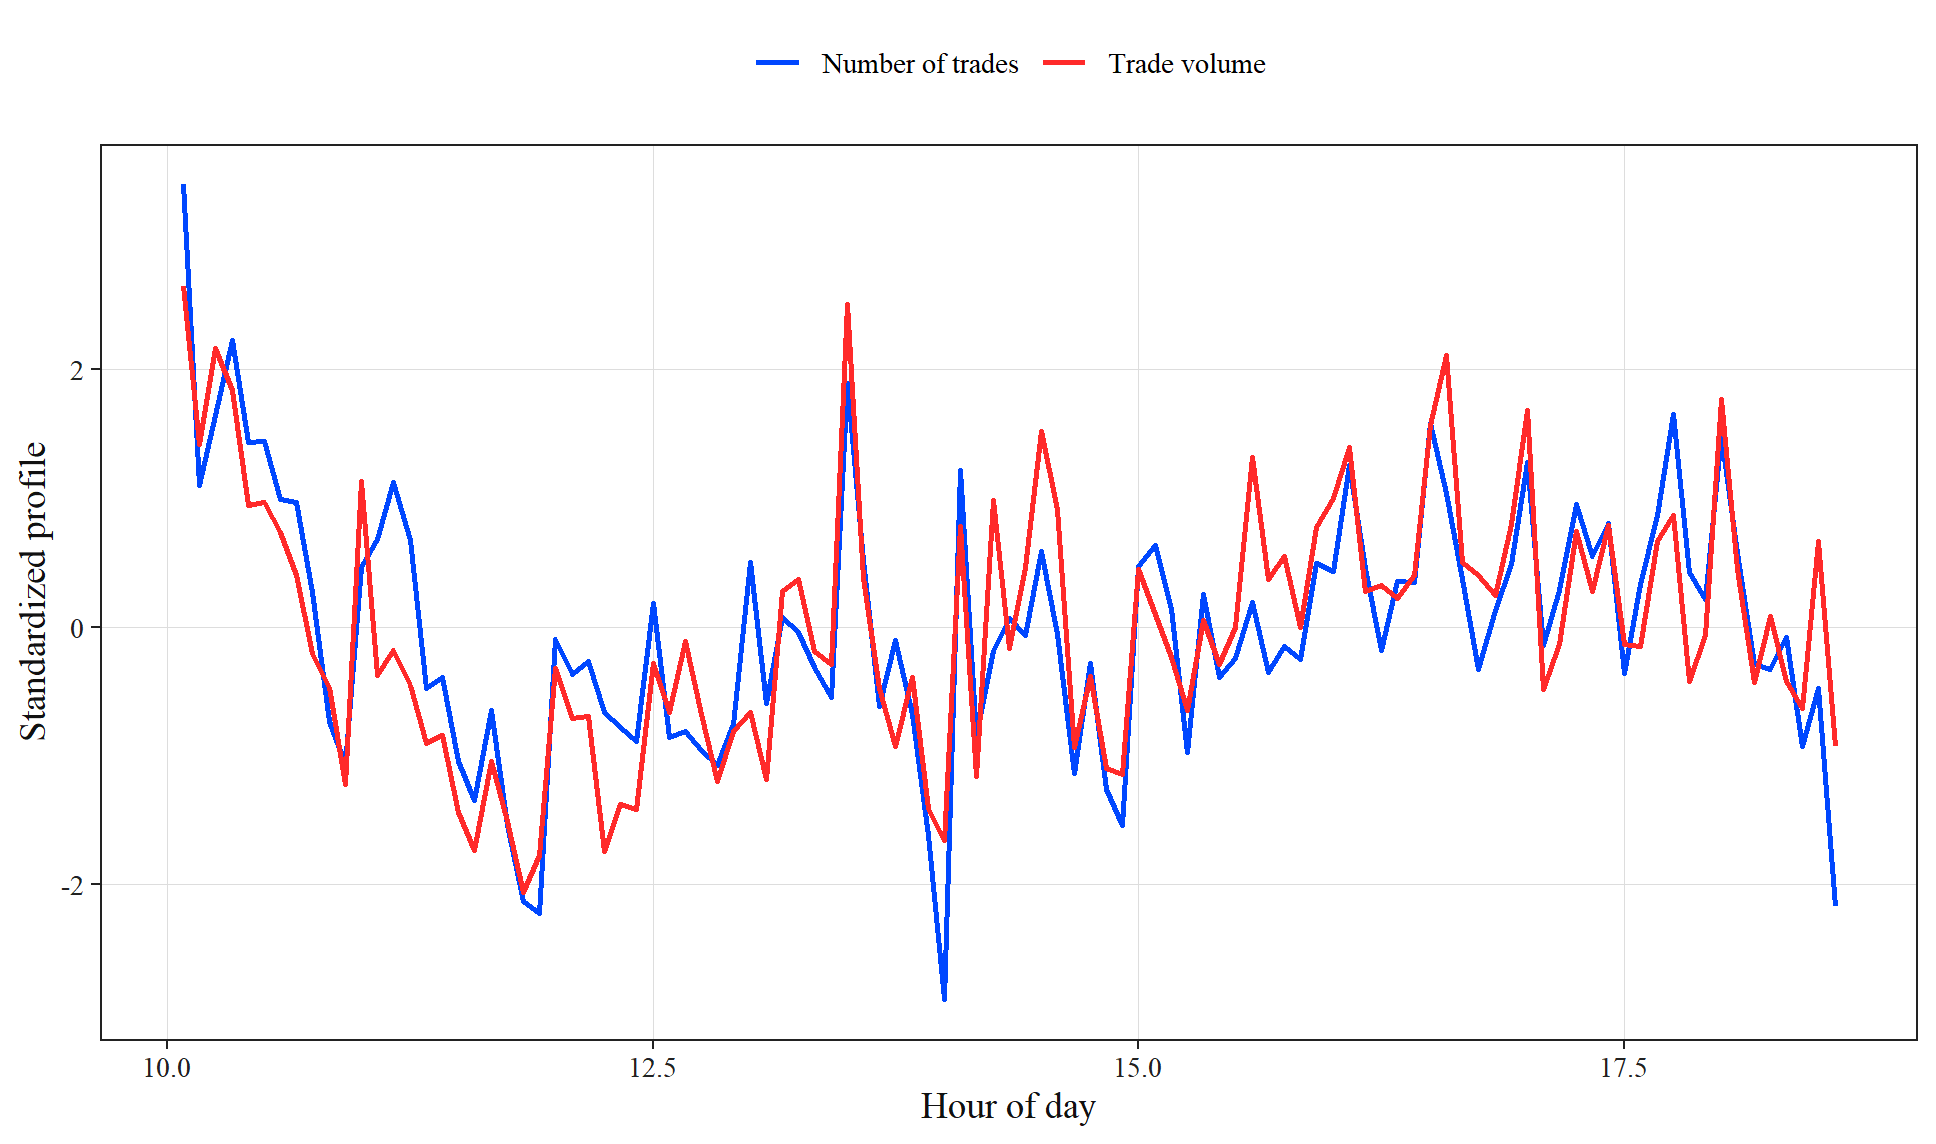
\includegraphics[width=\textwidth]{results/02_seasonality/intraday_trade_activity.png}
\caption{Trade activity}
\end{subfigure}
\caption{Intraday profiles before state estimation}
\caption*{\footnotesize\emph{Notes:} The 14:00 movement is caused by the MOEX intraday clearing interval. These raw profiles show why time-of-day adjustment is needed: without it, the HMM could confuse regular daily patterns with genuine liquidity regimes. Times are Moscow time.}
\label{fig:appendix_seasonality}
\end{figure}

\begin{figure}[!htbp]
\centering
\begin{subfigure}{0.48\textwidth}
\centering
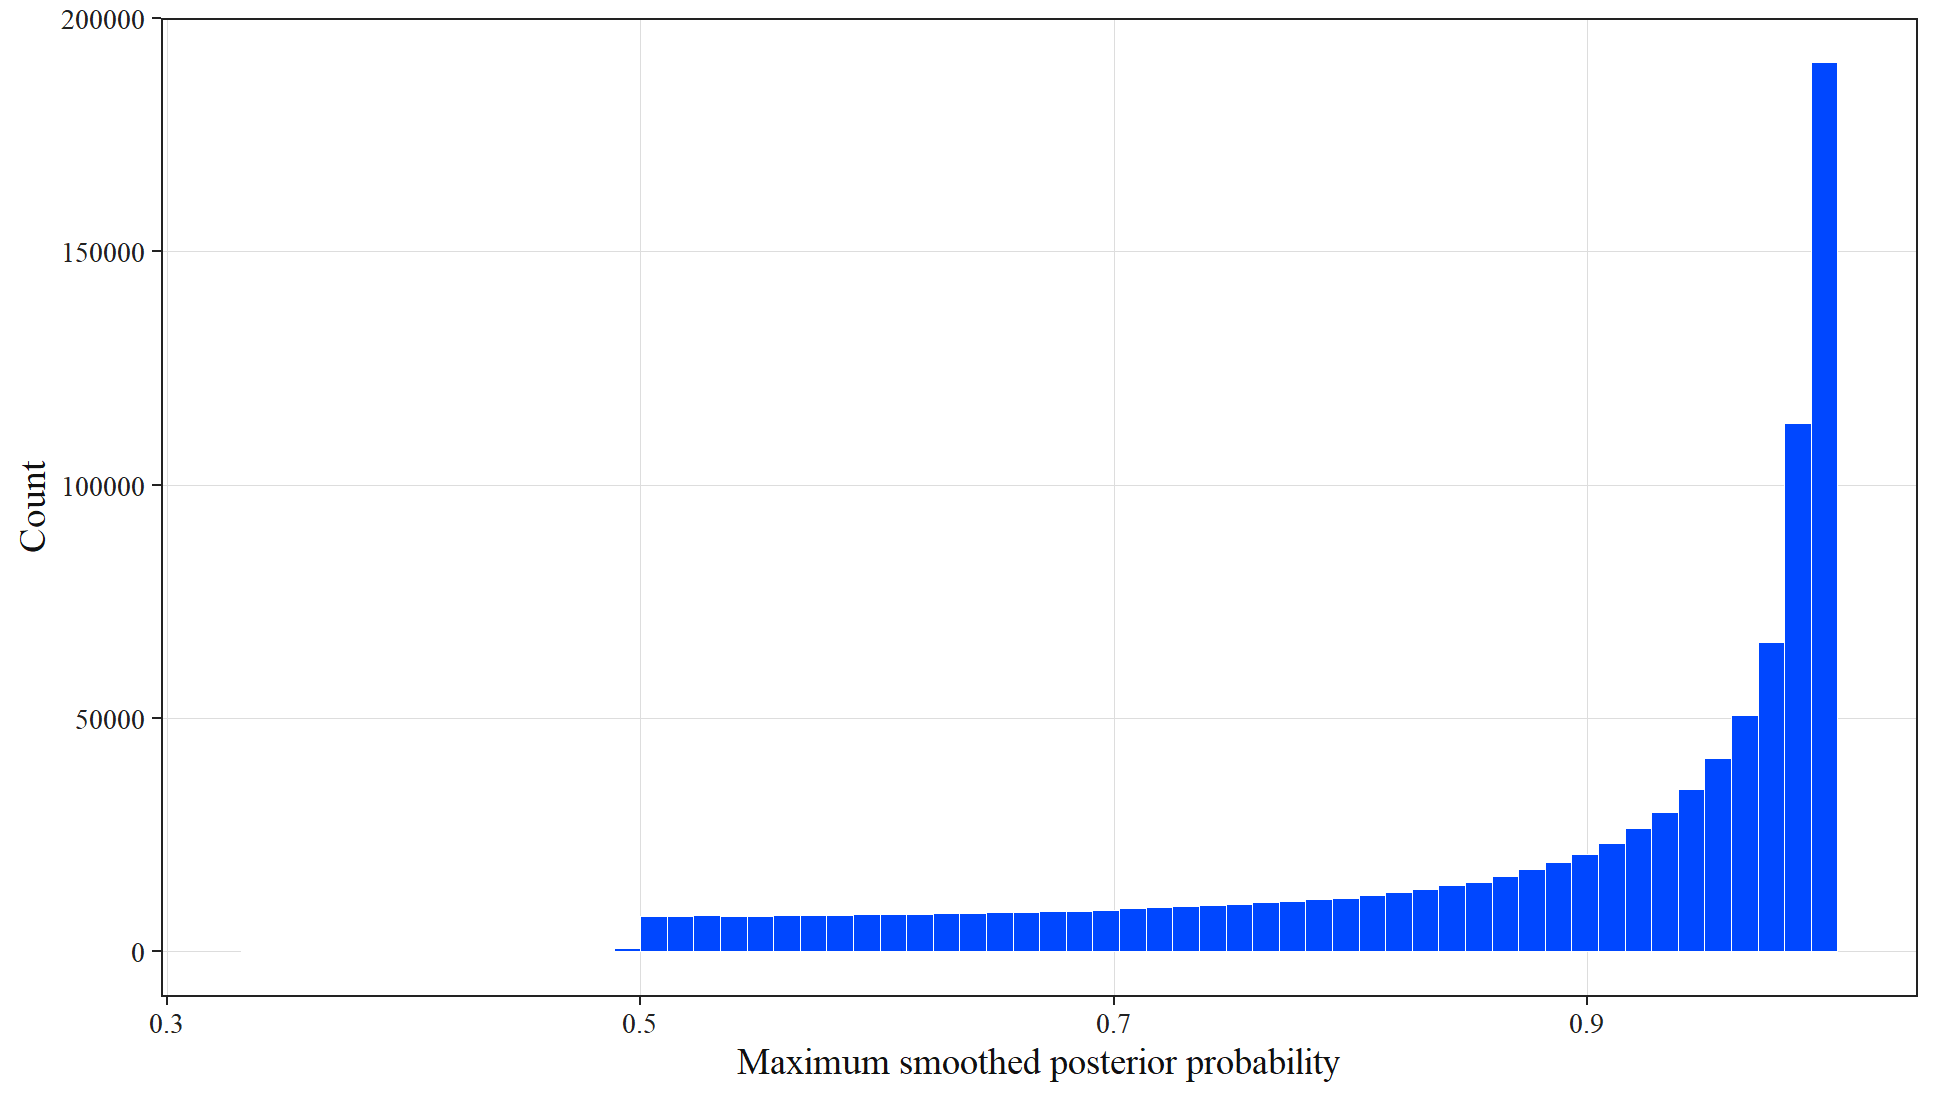
\includegraphics[width=\textwidth]{results/12_hmm_state_interpretation/maximum_posterior_histogram.png}
\caption{Classification confidence}
\end{subfigure}
\hfill
\begin{subfigure}{0.48\textwidth}
\centering
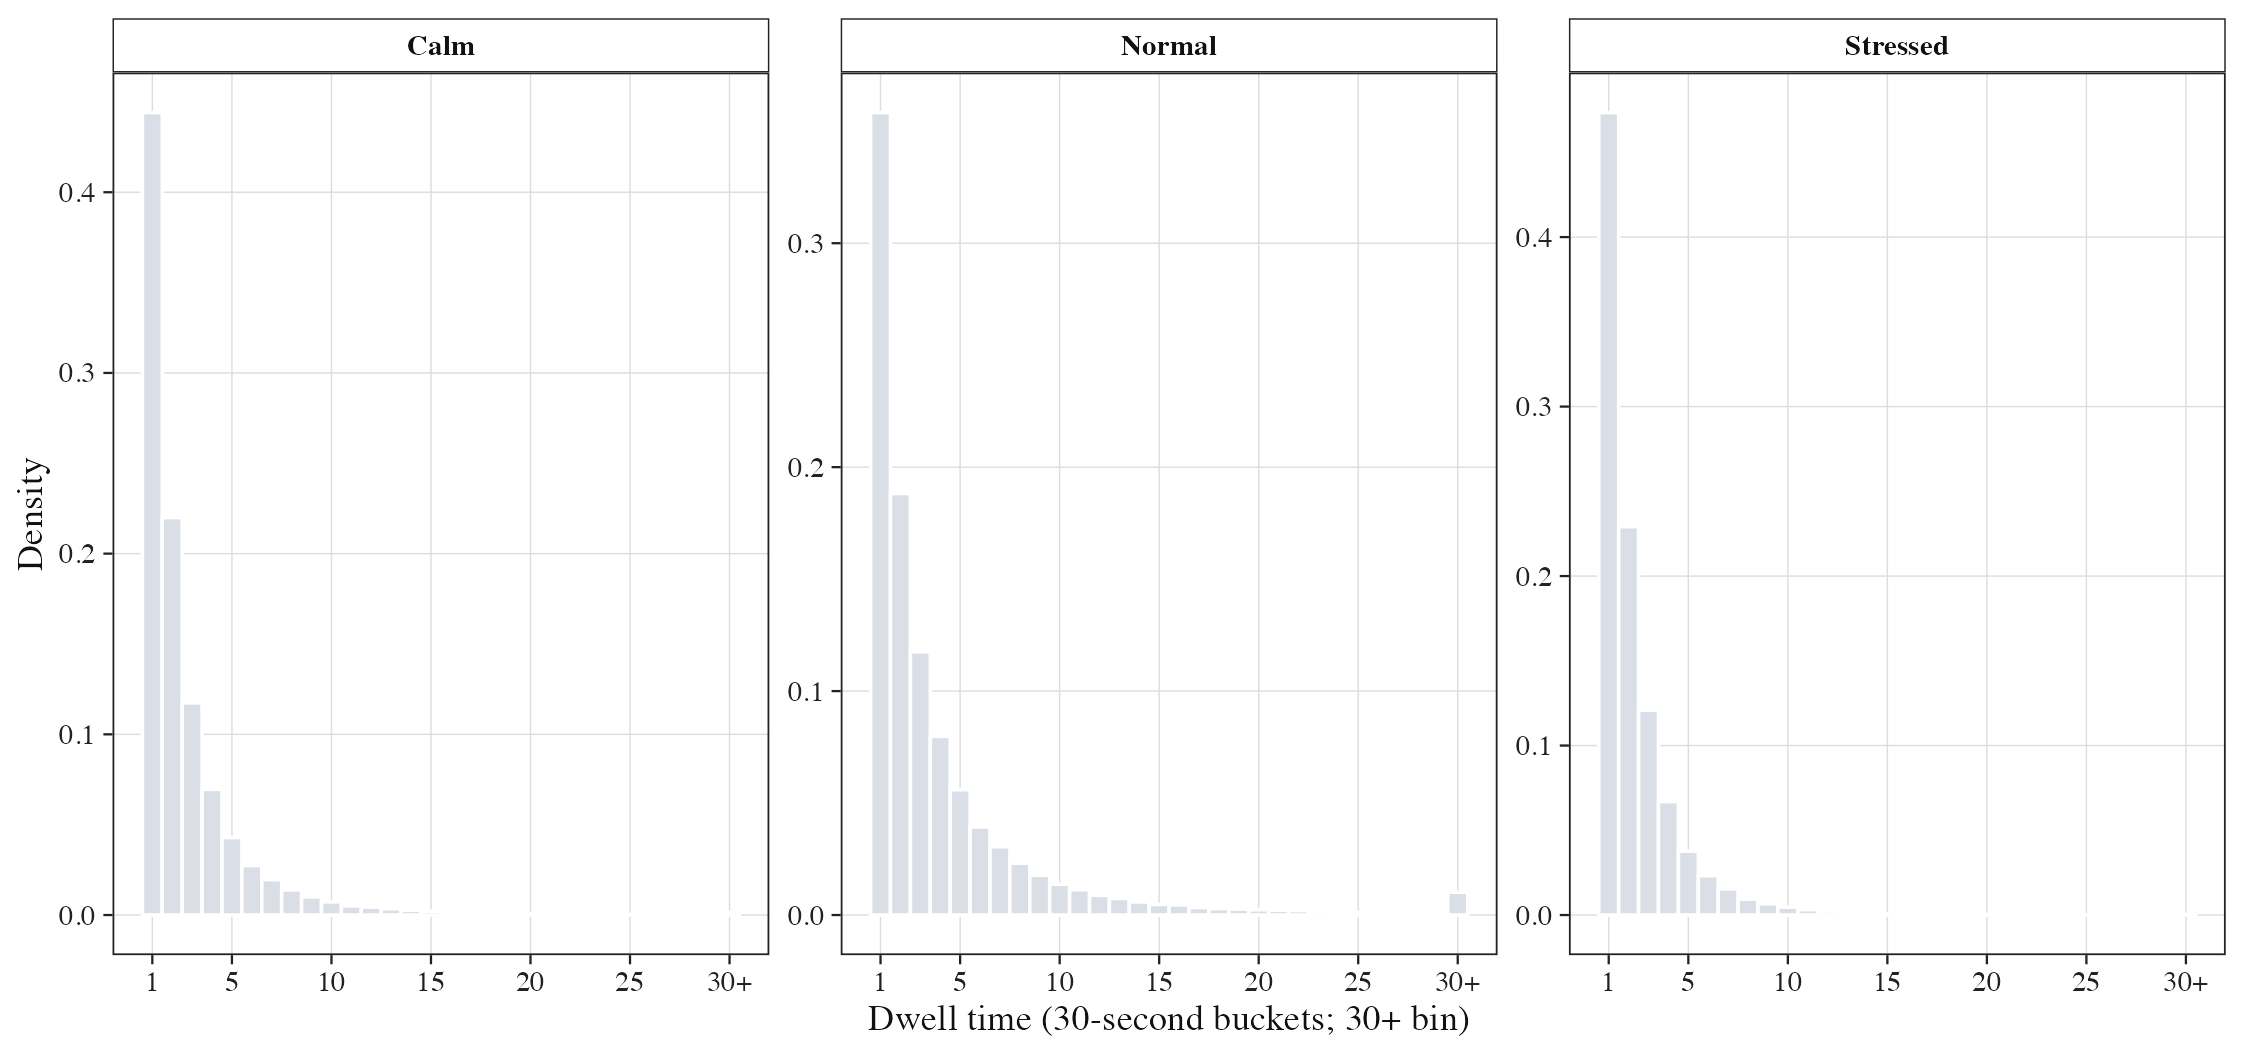
\includegraphics[width=\textwidth]{results/12_hmm_state_interpretation/dwell_time_histograms.png}
\caption{State dwell times}
\end{subfigure}
\caption{Supplementary classification diagnostics}
\caption*{\footnotesize\emph{Notes:} Panel (a) shows how confident the model is in its most likely state assignment for each bucket. Panel (b) shows how long decoded state episodes last, with longer episodes grouped at 30 buckets so the common short episodes remain visible. Together, the panels show that the states are useful but not perfectly certain, and that most episodes last minutes rather than hours.}
\label{fig:appendix_classification}
\end{figure}

\begin{figure}[!htbp]
\centering
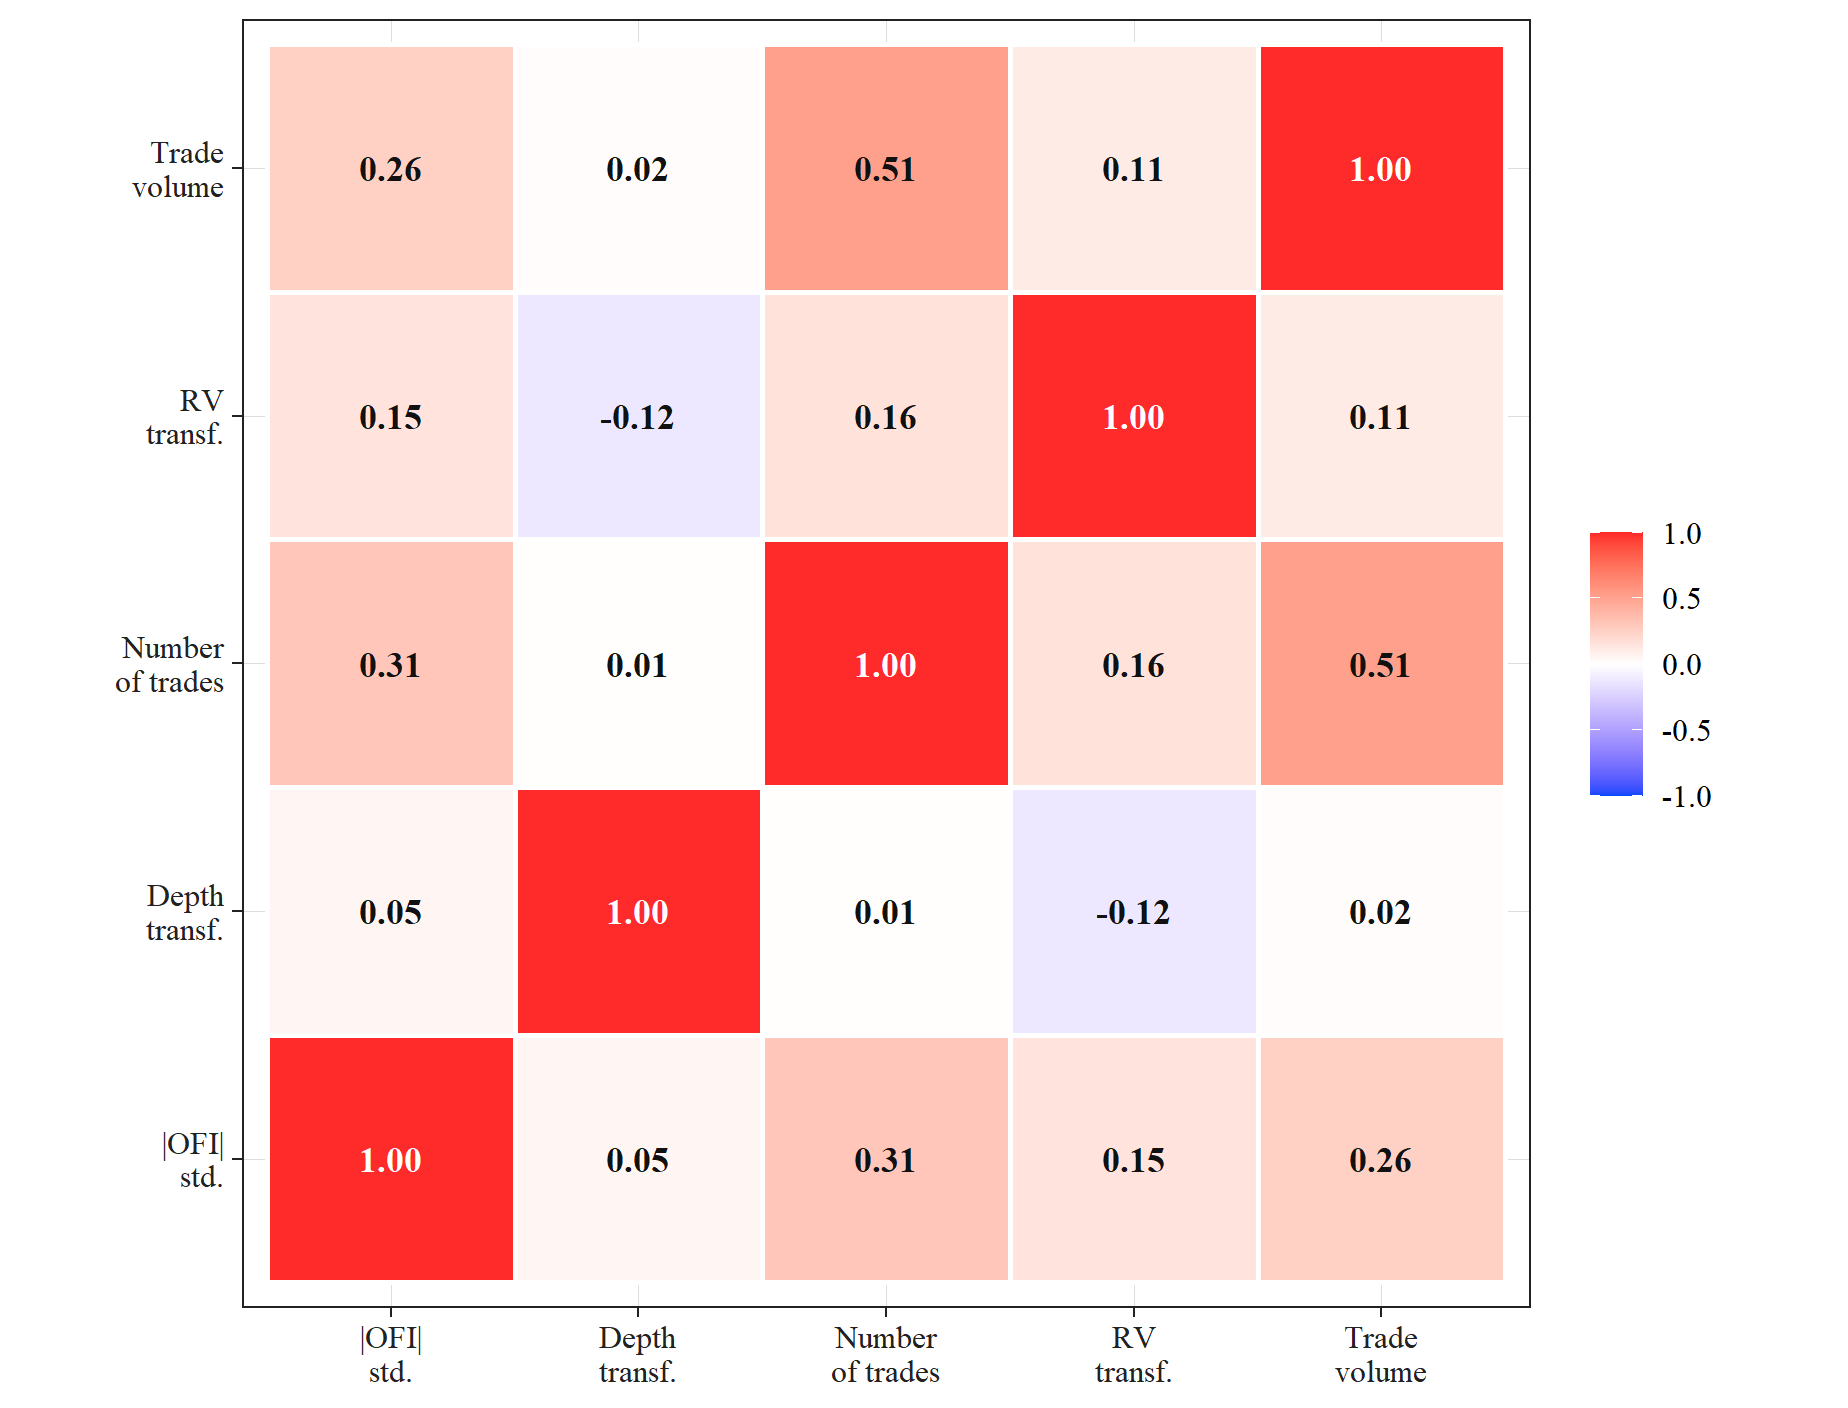
\includegraphics[width=0.70\textwidth]{results/05_regressors/regressor_correlation_heatmap.png}
\caption{Correlation heatmap for transition regressors}
\caption*{\footnotesize\emph{Notes:} This heatmap checks whether the transition regressors mostly repeat the same information. The correlations are not large enough to make the covariates redundant, so depth, realized volatility, absolute OFI pressure  and open/close indicators are kept as separate transition variables.}
\label{fig:appendix_regressor_heatmap}
\end{figure}

\FloatBarrier

\clearpage
\phantomsection
\addcontentsline{toc}{section}{References}
\begingroup
\raggedright
\begin{thebibliography}{99}

\bibitem[Andersen and Bollerslev(1997)]{AndersenBollerslev1997}
Andersen, T. G.  and Bollerslev, T. (1997).
\newblock Intraday periodicity and volatility persistence in financial markets.
\newblock \emph{Journal of Empirical Finance}, 4(2--3), 115--158.
\newblock \doi{10.1016/S0927-5398(97)00004-2}.

\bibitem[Brunnermeier and Pedersen(2009)]{BrunnermeierPedersen2009}
Brunnermeier, M. K.  and Pedersen, L. H. (2009).
\newblock Market liquidity and funding liquidity.
\newblock \emph{Review of Financial Studies}, 22(6), 2201--2238.
\newblock \doi{10.1093/rfs/hhn098}.

\bibitem[Cespa and Foucault(2014)]{CespaFoucault2014}
Cespa, G.  and Foucault, T. (2014).
\newblock Illiquidity contagion and liquidity crashes.
\newblock \emph{Review of Financial Studies}, 27(6), 1615--1660.
\newblock \doi{10.1093/rfs/hhu016}.

\bibitem[Chordia et al.(2000)]{ChordiaRollSubrahmanyam2000}
Chordia, T., Roll, R.  and Subrahmanyam, A. (2000).
\newblock Commonality in liquidity.
\newblock \emph{Journal of Financial Economics}, 56(1), 3--28.
\newblock \doi{10.1016/S0304-405X(99)00057-4}.

\bibitem[Cont et al.(2014)]{ContKukanovStoikov2014}
Cont, R., Kukanov, A.  and Stoikov, S. (2014).
\newblock The price impact of order book events.
\newblock \emph{Journal of Financial Econometrics}, 12(1), 47--88.
\newblock \doi{10.1093/jjfinec/nbt003}.

\bibitem[Cont et al.(2023)]{ContCucuringuZhang2023}
Cont, R., Cucuringu, M.  and Zhang, C. (2023).
\newblock Cross-impact of order flow imbalance in equity markets.
\newblock \emph{Quantitative Finance}, 23(10), 1373--1393.
\newblock \doi{10.1080/14697688.2023.2236159}.

\bibitem[Easley and O'Hara(1992)]{EasleyOHara1992}
Easley, D.  and O'Hara, M. (1992).
\newblock Time and the process of security price adjustment.
\newblock \emph{Journal of Finance}, 47(2), 577--605.
\newblock \doi{10.1111/j.1540-6261.1992.tb04402.x}.

\bibitem[Flood et al.(2016)]{FloodLiechtyPiontek2016}
Flood, M. D., Liechty, J.  and Piontek, T. (2016).
\newblock Systemwide commonalities in market liquidity.
\newblock Office of Financial Research Working Paper 15-11.
\newblock \url{https://www.financialresearch.gov/working-papers/2015/05/28/systemwide-commonalities-in-market-liquidity}.

\bibitem[Foucault et al.(2005)]{FoucaultKadanKandel2005}
Foucault, T., Kadan, O.  and Kandel, E. (2005).
\newblock Limit order book as a market for liquidity.
\newblock \emph{Review of Financial Studies}, 18(4), 1171--1217.
\newblock \doi{10.1093/rfs/hhi029}.

\bibitem[Glosten and Milgrom(1985)]{GlostenMilgrom1985}
Glosten, L. R.  and Milgrom, P. R. (1985).
\newblock Bid, ask and transaction prices in a specialist market with heterogeneously informed traders.
\newblock \emph{Journal of Financial Economics}, 14(1), 71--100.
\newblock \doi{10.1016/0304-405X(85)90044-3}.

\bibitem[Hamilton(1989)]{Hamilton1989}
Hamilton, J. D. (1989).
\newblock A new approach to the economic analysis of nonstationary time series and the business cycle.
\newblock \emph{Econometrica}, 57(2), 357--384.
\newblock \doi{10.2307/1912559}.

\bibitem[Hasbrouck(1991)]{Hasbrouck1991}
Hasbrouck, J. (1991).
\newblock Measuring the information content of stock trades.
\newblock \emph{Journal of Finance}, 46(1), 179--207.
\newblock \doi{10.1111/j.1540-6261.1991.tb03749.x}.

\bibitem[Kyle(1985)]{Kyle1985}
Kyle, A. S. (1985).
\newblock Continuous auctions and insider trading.
\newblock \emph{Econometrica}, 53(6), 1315--1335.
\newblock \doi{10.2307/1913210}.

\bibitem[Lee and Ready(1991)]{LeeReady1991}
Lee, C. M. C.  and Ready, M. J. (1991).
\newblock Inferring trade direction from intraday data.
\newblock \emph{Journal of Finance}, 46(2), 733--746.
\newblock \doi{10.1111/j.1540-6261.1991.tb02683.x}.

\bibitem[Meldrum and Sokolinskiy(2025)]{MeldrumSokolinskiy2025}
Meldrum, A.  and Sokolinskiy, O. (2025).
\newblock The relationship between market depth and liquidity fragility in the Treasury market.
\newblock Finance and Economics Discussion Series 2025-014, Board of Governors of the Federal Reserve System.
\newblock \doi{10.17016/FEDS.2025.014}.

\bibitem[MOEX(n.d.a)]{MOEXBlueChip}
Moscow Exchange. (n.d.a).
\newblock Blue Chip Index description page.
\newblock Accessed May 19, 2026.
\newblock \url{https://www.moex.com/a6447}.

\bibitem[MOEX(n.d.b)]{MOEXFullOrdersLog}
Moscow Exchange. (n.d.b).
\newblock Detailed file layout for Full Orders Log, type A.
\newblock Accessed May 19, 2026.
\newblock \url{https://www.moex.com/a1680}.

\bibitem[Nguyen et al.(2020)]{NguyenEngleFlemingGhysels2020}
Nguyen, G., Engle, R., Fleming, M. J.  and Ghysels, E. (2020).
\newblock Liquidity and volatility in the U.S. Treasury market.
\newblock \emph{Journal of Econometrics}, 217(2), 207--229.
\newblock \doi{10.1016/j.jeconom.2019.12.002}.

\bibitem[Raman et al.(2020)]{RamanRobeYadav2020}
Raman, V., Robe, M. A.  and Yadav, P. K. (2020).
\newblock Man vs. machine: Liquidity provision and market fragility.
\newblock Working paper, SSRN.
\newblock \doi{10.2139/ssrn.3757848}.

\bibitem[Xu et al.(2019)]{XuGouldHowison2019}
Xu, K., Gould, M. D.  and Howison, S. D. (2019).
\newblock Multi-level order-flow imbalance in a limit order book.
\newblock arXiv:1907.06230.
\newblock \url{https://arxiv.org/abs/1907.06230}.

\end{thebibliography}
\endgroup

\end{document}
